
%%
%% forked from https://gits-15.sys.kth.se/giampi/kthlatex kthlatex-0.2rc4 on 2020-02-13
%% expanded upon by Gerald Q. Maguire Jr.
%% This template has been adapted by Anders Sjögren to the University
%% Engineering Program in Computer Science at KTH ICT. This adaptation was
%% Many thanks to others who have provided constructive input regarding the template.

% Make it possible to conditionally depend on the TeX engine used
\RequirePackage{ifxetex}
\RequirePackage{ifluatex}
\newif\ifxeorlua
\ifxetex\xeorluatrue\fi
\ifluatex\xeorluatrue\fi

\ifxeorlua
% The following is to ensure that the PDF uses a recent version rather than the typical PDF 1-5
%  This same version of PDF should be set as an option for hyperef

\RequirePackage{expl3}
\ExplSyntaxOn
%pdf_version_gset:n{2.0}
%\pdf_version_gset:n{1.5}

%% Alternatively, if you have a LaTeX newer than June 2022, you can use the following. However, then you have to remove the pdfversion from hyperef. It also breaks hyperxmp. So perhaps it is too early to try using it!
%\DocumentMetadata
%{
%% testphase = phase-I, % tagging without paragraph tagging
% testphase = phase-II % tagging with paragraph tagging and other new stuff.
%pdfversion = 2.0 % pdfversion must be set here.
%}

% Optionally, you can set the uncompress flag to make it easier to examine the PDF
%\pdf_uncompress: % to check the pdf
\ExplSyntaxOff
\else
\RequirePackage{expl3}
\ExplSyntaxOn
%\pdf_version_gset:n{2.0}
\pdf_version_gset:n{1.5}
\ExplSyntaxOff
\fi

%% Define a pair of commands to disable and reenable specific packages - see https://tex.stackexchange.com/questions/39415/unload-a-latex-package
\makeatletter
\newcommand{\disablepackage}[2]{%
  \disable@package@load{#1}{#2}%
}
\newcommand{\reenablepackage}[1]{%
  \reenable@package@load{#1}%
}
\makeatother
%% To avoid the warning: "Package transparent Warning: Loading aborted, because pdfTeX is not running in PDF mode."
\ifxeorlua
\disablepackage{transparent}{}
\fi



%% The template is designed to handle a thesis in English or Swedish
% set the default language to english or swedish by passing an option to the documentclass - this handles the inside title page
% To optimize for digital output (this changes the color palette add the option: digitaloutput
% To use \ifnomenclature add the option nomenclature
% To use bibtex or biblatex - include one of these as an option
\documentclass[nomenclature, english, bibtex]{kththesis}
%\documentclass[swedish, biblatex]{kththesis}
% if pdflatex \usepackage[utf8]{inputenc}


%% Conventions for todo notes:
% Informational
%% \generalExpl{Comments/directions/... in English}
\newcommand*{\generalExpl}[1]{\todo[inline]{#1}}

% Language-specific information (currently in English or Swedish)
\newcommand*{\engExpl}[1]{\todo[inline, backgroundcolor=kth-lightgreen40]{#1}} %% \engExpl{English descriptions about formatting}
\newcommand*{\sweExpl}[1]{\todo[inline, backgroundcolor=kth-lightblue40]{#1}}  %% % \sweExpl{Text på svenska}

% warnings
\newcommand*{\warningExpl}[1]{\todo[inline, backgroundcolor=kth-lightred40]{#1}} %% \warningExpl{warnings}

% Uncomment to hide specific comments, to hide **all** ToDos add `final` to
% document class
% \renewcommand\warningExpl[1]{}
% \renewcommand\generalExpl[1]{}
% \renewcommand\engExpl[1]{}
% For example uncommenting the following line hides the Swedish language explanations
% \renewcommand\sweExpl[1]{}


% \usepackage[style=numeric,sorting=none,backend=biber]{biblatex}
\ifbiblatex
    %\usepackage[language=english,bibstyle=authoryear,citestyle=authoryear, maxbibnames=99]{biblatex}
    % Alternatively you might use another style, such as IEEE and use citestyle=numeric-comp  to put multiple citations in a single pair of square brackets
    \usepackage[style=ieee,citestyle=numeric-comp]{biblatex}
    \addbibresource{references}
    %\DeclareLanguageMapping{norsk}{norwegian}
\else
    % The line(s) below are for BibTeX
    \bibliographystyle{bibstyle/myIEEEtran}
    %\bibliographystyle{apalike}
\fi


% include a variety of packages that are useful
\input{lib/includes}
\input{lib/kthcolors}

%\glsdisablehyper
%\makeglossaries
%\makenoidxglossaries
%%%% Local Variables:
%%% mode: latex
%%% TeX-master: t
%%% End:
% The following command is used with glossaries-extra
\setabbreviationstyle[acronym]{long-short}
% The form of the entries in this file is \newacronym{label}{acronym}{phrase}
%                                      or \newacronym[options]{label}{acronym}{phrase}
% see "User Manual for glossaries.sty" for the  details about the options, one example is shown below
% note the specification of the long form plural in the line below
% \newacronym[longplural={Debugging Information Entities}]{DIE}{DIE}{Debugging Information Entity}
%
% The following example also uses options
% \newacronym[shortplural={OSes}, firstplural={operating systems (OSes)}]{OS}{OS}{operating system}

% note the use of a non-breaking dash in long text for the following acronym
% \newacronym{IQL}{IQL}{Independent Q‑Learning}

% example of putting in a trademark on first expansion
% \newacronym[first={NVIDIA OpenSHMEM Library (NVSHMEM\texttrademark)}]{NVSHMEM}{NVSHMEM}{NVIDIA OpenSHMEM Library}

\newacronym{KTH}{KTH}{KTH Royal Institute of Technology}

\newacronym{DR}{DR}{Digital Radiography}
\newacronym{PR}{PR}{Projectional Radiography}
\newacronym{FSR}{FSR}{Film-Screen Radiography}

\newacronym{DIP}{DIP}{Digital Image Processing}
\newacronym{LUT}{LUT}{Look-Up-Table}

\newacronym{MSE}{MSE}{Mean Square Error}
\newacronym{TV}{TV}{Total Variation}
\newacronym{TGV}{TGV}{Total Generalized Variation}

\newa
                %load the acronyms file

\input{lib/defines}  % load some additional definitions to make writing more consistent

% The following is needed in conjunction with generating the DiVA data with abstracts and keywords using the scontents package and a modified listings environment
%\usepackage{listings}   %  already included
\ExplSyntaxOn
\newcommand\typestoredx[2]{\expandafter\__scontents_typestored_internal:nn\expandafter{#1} {#2}}
\ExplSyntaxOff
\makeatletter
\let\verbatimsc\@undefined
\let\endverbatimsc\@undefined
\lst@AddToHook{Init}{\hyphenpenalty=50\relax}
\makeatother


\lstnewenvironment{verbatimsc}
    {
    \lstset{%
        basicstyle=\ttfamily\tiny,
        backgroundcolor=\color{white},
        %basicstyle=\tiny,
        %columns=fullflexible,
        columns=[l]fixed,
        language=[LaTeX]TeX,
        %numbers=left,
        %numberstyle=\tiny\color{gray},
        keywordstyle=\color{red},
        breaklines=true,                 % sets automatic line breaking
        breakatwhitespace=true,          % sets if automatic breaks should only happen at whitespace
        %keepspaces=false,
        breakindent=0em,
        %fancyvrb=true,
        frame=none,                     % turn off any box
        postbreak={}                    % turn off any hook arrow for continuation lines
    }
}{}

%% Add some more keywords to bring out the structure more
\lstdefinestyle{[LaTeX]TeX}{
morekeywords={begin, todo, textbf, textit, texttt}
}

%% definition of new command for bytefield package
\newcommand{\colorbitbox}[3]{%
	\rlap{\bitbox{#2}{\color{#1}\rule{\width}{\height}}}%
	\bitbox{#2}{#3}}




% define a left aligned table cell that is ragged right
\newcolumntype{L}[1]{>{\raggedright\let\newline\\\arraybackslash\hspace{0pt}}p{#1}}

% Because backref is not compatible with biblatex
\ifbiblatex
    \usepackage[plainpages=false]{hyperref}
\else
    \usepackage[
    backref=page,
    pagebackref=false,
    plainpages=false,
                            % PDF related options
    unicode=true,           % Unicode encoded PDF strings
    bookmarks=true,         % generate bookmarks in PDF files
    bookmarksopen=false,    % Do not automatically open the bookmarks in the PDF reading program
    pdfpagemode=UseNone,    % None, UseOutlines, UseThumbs, or FullScreen
    destlabel,              % better naming of destinations
    pdfencoding=auto,       % for unicode in
    ]{hyperref}
    \makeatletter
    \ltx@ifpackageloaded{attachfile2}{
    % cannot use backref if one is using attachfile
    }
    {\usepackage{backref}
    %
    % Customize list of backreferences.
    % From https://tex.stackexchange.com/a/183735/1340
    \renewcommand*{\backref}[1]{}
    \renewcommand*{\backrefalt}[4]{%
    \ifcase #1%
          \or [Page~#2.]%
          \else [Pages~#2.]%
    \fi%
    }
    }
    \makeatother

\fi
\usepackage[all]{hypcap}	%% prevents an issue related to hyperref and caption linking

%% Acronyms
% note that nonumberlist - removes the cross references to the pages where the acronym appears
% note that super will set the descriptions text aligned
% note that nomain - does not produce a main glossary, thus only acronyms will be in the glossary
% note that nopostdot - will prevent there being a period at the end of each entry
\usepackage[acronym, style=super, section=section, nonumberlist, nomain,
nopostdot]{glossaries}
\setlength{\glsdescwidth}{0.75\textwidth}
\usepackage[]{glossaries-extra}
\ifinswedish
    %\usepackage{glossaries-swedish}
\fi

%% For use with the README_notes
% Define a new type of glossary so that the acronyms defined in the README_notes document can be distinct from those in the thesis template
% the tlg, tld, and dn will be the file extensions used for this glossary
\newglossary[tlg]{readme}{tld}{tdn}{README acronyms}


\input{lib/includes-after-hyperref}

%\glsdisablehyper
\makeglossaries
%\makenoidxglossaries

% The following bit of ugliness is because of the problems PDFLaTeX has handling a non-breaking hyphen
% unless it is converted to UTF-8 encoding.
% If you do not use such characters in your acronyms, this could be simplified to just include the acronyms file.
\ifxeorlua
%%% Local Variables:
%%% mode: latex
%%% TeX-master: t
%%% End:
% The following command is used with glossaries-extra
\setabbreviationstyle[acronym]{long-short}
% The form of the entries in this file is \newacronym{label}{acronym}{phrase}
%                                      or \newacronym[options]{label}{acronym}{phrase}
% see "User Manual for glossaries.sty" for the  details about the options, one example is shown below
% note the specification of the long form plural in the line below
% \newacronym[longplural={Debugging Information Entities}]{DIE}{DIE}{Debugging Information Entity}
%
% The following example also uses options
% \newacronym[shortplural={OSes}, firstplural={operating systems (OSes)}]{OS}{OS}{operating system}

% note the use of a non-breaking dash in long text for the following acronym
% \newacronym{IQL}{IQL}{Independent Q‑Learning}

% example of putting in a trademark on first expansion
% \newacronym[first={NVIDIA OpenSHMEM Library (NVSHMEM\texttrademark)}]{NVSHMEM}{NVSHMEM}{NVIDIA OpenSHMEM Library}

\newacronym{KTH}{KTH}{KTH Royal Institute of Technology}

\newacronym{DR}{DR}{Digital Radiography}
\newacronym{PR}{PR}{Projectional Radiography}
\newacronym{FSR}{FSR}{Film-Screen Radiography}

\newacronym{DIP}{DIP}{Digital Image Processing}
\newacronym{LUT}{LUT}{Look-Up-Table}

\newacronym{MSE}{MSE}{Mean Square Error}
\newacronym{TV}{TV}{Total Variation}
\newacronym{TGV}{TGV}{Total Generalized Variation}

\newa
                %load the acronyms file
\else
\input{lib/acronyms-for-pdflatex}
\fi


% insert the configuration information with author(s), examiner, supervisor(s), ...
\input{custom_configuration}

\title{Chest X-ray Transmission Map Reconstruction}
\subtitle{Regularizing Inverse Problems Through Domain Knowledge of Radiographic Image Processing}

% give the alternative title - i.e., if the thesis is in English, then give a Swedish title
\alttitle{Rekonstruktion av röntgenbild av bröstkorgen}
\altsubtitle{Reglering av inversa problem genom domänkunskap om radiografisk bildbehandling}
% alternative, if the thesis is in Swedish, then give an English title
%\alttitle{This is the English translation of the title}
%\altsubtitle{This is the English translation of the subtitle}

% Enter the English and Swedish keywords here for use in the PDF metadata _and_ for later use
% following the respective abstract.
% Try to put the words in the same order in both languages to facilitate matching. For example:
\EnglishKeywords{Nonlinear Optimization, Medical Imaging, Digital Image Processing, Chest X-ray, Inverse Problems, Constrained Optimization}
\SwedishKeywords{Icke-linjär optimering, Medicinsk bildvetenskap, digital bildbehandling, Lungröntgen, Inversa problem, Begränsad optimering}

%%%%% For the oral presentation
%% Add this information once your examiner has scheduled your oral presentation
\presentationDateAndTimeISO{2022-03-15 13:00}
\presentationLanguage{eng}
\presentationRoom{via Zoom https://kth-se.zoom.us/j/ddddddddddd}
\presentationAddress{Isafjordsgatan 22 (Kistagången 16)}
\presentationCity{Stockholm}

% When there are multiple opponents, separate their names with '\&'
% Opponent's information
\opponentsNames{A. B. Normal \& A. X. E. Normalè}

% Once a thesis is approved by the examiner, add the TRITA number
% The TRITA number for a thesis consists of two parts: a series (unique to each school)
% and the number in the series, which is formatted as the year followed by a colon and
% then a unique series number for the thesis - starting with 1 each year.
\trita{TRITA -- EECS-EX}{2024:0000}

% Put the title, author, and keyword information into the PDF meta information
\input{lib/pdf_related_includes}


% the custom colors and the commands are defined in defines.tex
\hypersetup{
	colorlinks  = true,
	breaklinks  = true,
	linkcolor   = \linkscolor,
	urlcolor    = \urlscolor,
	citecolor   = \refscolor,
	anchorcolor = black
}

\ifnomenclature
% The following lines make the page numbers and equations hyperlinks in the Nomenclature list
\renewcommand*{\pagedeclaration}[1]{\unskip, \dotfill\hyperlink{page.#1}{page\nobreakspace#1}}
% The following does not work correctly, as the name of the cross-reference is incorrect
%\renewcommand*{\eqdeclaration}[1]{, see equation\nobreakspace(\hyperlink{equation.#1}{#1})}

% You can also change the page heading for the nomenclature
\renewcommand{\nomname}{List of Symbols Used}

% You can even add customization text before the list
\renewcommand{\nompreamble}{The following symbols will be later used within the body of the thesis.}
\makenomenclature
\fi

%
% The commands below are to configure JSON listings
%
% format for JSON listings
\colorlet{punct}{red!60!black}
\definecolor{delim}{RGB}{20,105,176}
\definecolor{numb}{RGB}{106, 109, 32}
\definecolor{string}{RGB}{0, 0, 0}

\lstdefinelanguage{json}{
    numbers=none,
    numberstyle=\small,
    frame=none,
    rulecolor=\color{black},
    showspaces=false,
    showtabs=false,
    breaklines=true,
    postbreak=\raisebox{0ex}[0ex][0ex]{\ensuremath{\color{gray}\hookrightarrow\space}},
    breakatwhitespace=true,
    basicstyle=\ttfamily\small,
    extendedchars=false,
    upquote=true,
    morestring=[b]",
    stringstyle=\color{string},
    literate=
     *{0}{{{\color{numb}0}}}{1}
      {1}{{{\color{numb}1}}}{1}
      {2}{{{\color{numb}2}}}{1}
      {3}{{{\color{numb}3}}}{1}
      {4}{{{\color{numb}4}}}{1}
      {5}{{{\color{numb}5}}}{1}
      {6}{{{\color{numb}6}}}{1}
      {7}{{{\color{numb}7}}}{1}
      {8}{{{\color{numb}8}}}{1}
      {9}{{{\color{numb}9}}}{1}
      {:}{{{\color{punct}{:}}}}{1}
      {,}{{{\color{punct}{,}}}}{1}
      {\{}{{{\color{delim}{\{}}}}{1}
      {\}}{{{\color{delim}{\}}}}}{1}
      {[}{{{\color{delim}{[}}}}{1}
      {]}{{{\color{delim}{]}}}}{1}
      {’}{{\char13}}1,
}

\lstdefinelanguage{XML}
{
  basicstyle=\ttfamily\color{blue}\bfseries\small,
  morestring=[b]",
  morestring=[s]{>}{<},
  morecomment=[s]{<?}{?>},
  stringstyle=\color{black},
  identifierstyle=\color{blue},
  keywordstyle=\color{cyan},
  breaklines=true,
  postbreak=\raisebox{0ex}[0ex][0ex]{\ensuremath{\color{gray}\hookrightarrow\space}},
  breakatwhitespace=true,
  morekeywords={xmlns,version,type}% list your attributes here
}

% If you use both listing and lstlisting environments - the following makes them both use the same counter and the same formatting in the List of Listings
\makeatletter
\AtBeginDocument{\let\c@listing\c@lstlisting}
\AtBeginDocument{\let\l@listing\l@lstlisting}
\makeatother

% Change the heading for the "List of Listings" to simply "Listings"
\renewcommand{\lstlistlistingname}{Listings}

% number each listing within the chapter
\numberwithin{listing}{chapter}

\usepackage{subfiles}

% To have Creative Commons (CC) license and logos use the doclicense package
% Note that the lowercase version of the license has to be used in the modifier
% i.e., one of by, by-nc, by-nd, by-nc-nd, by-sa, by-nc-sa, zero.
% For background see:
% https://www.kb.se/samverkan-och-utveckling/oppen-tillgang-och-bibsamkonsortiet/open-access-and-bibsam-consortium/open-access/creative-commons-faq-for-researchers.html
% https://kib.ki.se/en/publish-analyse/publish-your-article-open-access/open-licence-your-publication-cc
\begin{comment}
\usepackage[
    type={CC},
    %modifier={by-nc-nd},
    %version={4.0},
    modifier={by-nc},
    imagemodifier={-eu-88x31},  % to get Euro symbol rather than Dollar sign
    hyphenation={RaggedRight},
    version={4.0},
    %modifier={zero},
    %version={1.0},
]{doclicense}
\end{comment}

\begin{document}
%\selectlanguage{swedish}
%
\selectlanguage{english}

%%% Set the numbering for the title page to a numbering series not in the preface or body
\pagenumbering{alph}
\kthcover
\clearpage\thispagestyle{empty}\mbox{} % empty back of front cover
\titlepage

% If you do not want to have a bookinfo page, comment out the line saying \bookinfopage and add a \cleardoublepage
% If you want a bookinfo page: you will get a copyright notice, unless you have used the doclicense package in which case you will get a Creative Commons license. To include the doclicense package, uncomment the configuration of this package above and configure it with your choice of license.
\bookinfopage

% Frontmatter includes the abstracts and table-of-contents
\frontmatter
\setcounter{page}{1}
\begin{abstract}
% The first abstract should be in the language of the thesis.
% Abstract fungerar på svenska också.
  \markboth{\abstractname}{}
\begin{scontents}[store-env=lang]
eng
\end{scontents}
%%% The contents of the abstract (between the begin and end of scontents) will be saved in LaTeX format
%%% and output on the page(s) at the end of the thesis with information for DiVA facilitating the correct
%%% entry of the meta data for your thesis.
%%% These page(s) will be removed before the thesis is inserted into DiVA.
% ----- EXPLANATION -----
% \engExpl{All theses at KTH are \textbf{required} to have an abstract in both \textit{English} and \textit{Swedish}.}

% \engExpl{Exchange students may want to include one or more abstracts in the language(s) used in their home institutions to avoid the need to write another thesis when returning to their home institution.}

% \generalExpl{Keep in mind that most of your potential readers are only going to read your \texttt{title} and \texttt{abstract}. This is why the abstract must give them enough information so that they can decide if this document is relevant to them or not. Otherwise, the likely default choice is to ignore the rest of your document.\\
% An abstract should stand on its own, \ie no citations, cross-references to the body of the document, acronyms must be spelled out, \ldots .\\Write this early and revise as necessary. This will help keep you focused on what you are trying to do.}

\begin{scontents}[store-env=abstracts,print-env=true]
% % \generalExpl{Enter your abstract here!}
% An abstract is (typically) about 250 and 350 words (1/2 A4-page) with the following components:
% % key parts of the abstract
% \begin{itemize}
%   \item What is the topic area? (optional) Introduces the subject area for the project.
%   \item Short problem statement
%   \item Why was this problem worth a Bachelor's/Master’s thesis project? (\ie, why is the problem both significant and of a suitable degree of difficulty for a Bachelor's/Master’s thesis project? Why has no one else solved it yet?)
%   \item How did you solve the problem? What was your method/insight?
%   \item Results/Conclusions/Consequences/Impact: What are your key results/\linebreak[4]conclusions? What will others do based on your results? What can be done now that you have finished - that could not be done before your thesis project was completed?
% \end{itemize}

Chest X-ray datasets exhibit significant appearance variability due to diverse acquisition systems and proprietary image processing pipelines across manufacturers, limiting the generalizability of learning models. This variability particularly affects alternative X-ray detectors that are underrepresented in major datasets like CheXpert and ChestX-ray8, hindering the development of diagnostic tools for, for instance, resource-limited settings where such systems are essential.
This thesis addresses the challenge of recovering transmission maps—the fundamental physical measurements representing the fraction of incident X-ray radiation transmitted through the patient—from processed clinical images. Transmission maps are the raw measurements common to all X-ray detectors before manufacturer-specific processing, making them ideal detector-agnostic representations for machine learning applications.
The primary challenge is the absence of paired transmission map and processed image data, as manufacturers do not typically provide access to raw detector outputs, and is neither a tool directly used by radiologists to do diagnoses. Combined with the proprietary and non-linear nature of image processing algorithms, this creates an ill-posed inverse problem that has not been previously addressed. Without ground truth data, conventional supervised learning approaches are infeasible.
A framework to simulate transmission is proposed in the form of a solution for a constrained non-linear optimization method. The method leverages knowledge of common image processing operations in x-ray images to constrain the solution space. By incorporating anatomical priors based on the known attenuation properties of different tissue types, the problem can be conditioned to yield physically plausible solutions despite the lack of training data.
The method successfully recovers transmission maps that satisfies empirical expectations
from such images and that can be mapped back into their processed versions.
\end{scontents}

\subsection*{Keywords}
\begin{scontents}[store-env=keywords,print-env=true]
% If you set the EnglishKeywords earlier, you can retrieve them with:
\InsertKeywords{english}
% If you did not set the EnglishKeywords earlier then simply enter the keywords here:
% comma separate keywords, such as: Canvas Learning Management System, Docker containers, Performance tuning
\end{scontents}

\end{abstract}
\cleardoublepage
\babelpolyLangStart{swedish}
\begin{abstract}
    \markboth{\abstractname}{}
\begin{scontents}[store-env=lang]
swe
\end{scontents}
% \warningExpl{Inside the following scontents environment, you cannot use a \textbackslash include{filename} as the command rather than the file contents will end up in the for DiVA information. Additionally, you should not use a straight double quote character in the abstracts or keywords, use two single quote characters instead.}
\begin{scontents}[store-env=abstracts,print-env=true]
Dataset för röntgenbilder av bröstkorgen uppvisar betydande variationer i utseende på grund av olika insamlingssystem och proprietära bildbehandlingspipelines hos olika tillverkare, vilket begränsar generaliserbarheten hos inlärningsmodeller. Denna variation påverkar särskilt alternativa röntgendetektorer som är underrepresenterade i stora dataset som CheXpert och ChestX-ray8, vilket hindrar utvecklingen av diagnostiska verktyg för exempelvis resursbegränsade miljöer där sådana system är nödvändiga.
Denna avhandling behandlar utmaningen att återställa transmissionskartor – de grundläggande fysiska mätningarna som representerar andelen av den infallande röntgenstrålningen som transmitteras genom patienten – från bearbetade kliniska bilder. Transmissionskartor är de råa mätningar som är gemensamma för alla röntgendetektorer före tillverkarspecifik bearbetning, vilket gör dem till idealiska detektoroberoende representationer för maskininlärningsapplikationer.
Den främsta utmaningen är avsaknaden av parade transmissionskartor och bearbetade bilddata, eftersom tillverkare vanligtvis inte ger tillgång till råa detektorutdata, och det är inte heller ett verktyg som radiologer använder direkt för att ställa diagnoser. I kombination med den proprietära och icke-linjära karaktären hos bildbearbetningsalgoritmer skapar detta ett illa formulerat invers problem som inte har behandlats tidigare. Utan grundläggande sanningsdata är konventionella övervakade inlärningsmetoder omöjliga.
Ett ramverk för att simulera transmission föreslås i form av en lösning för en begränsad icke-linjär optimeringsmetod. Metoden utnyttjar kunskap om vanliga bildbehandlingsoperationer i röntgenbilder för att begränsa lösningsutrymmet. Genom att införliva anatomiska förkunskaper baserade på kända dämpningsegenskaper hos olika vävnadstyper kan problemet konditioneras för att ge fysiskt rimliga lösningar trots bristen på träningsdata.
Metoden återställer framgångsrikt transmissionskartor som uppfyller empiriska förväntningar
från sådana bilder och som kan mappas tillbaka till sina bearbetade versioner.

% \sweExpl{Alla avhandlingar vid KTH \textbf{måste ha} ett abstrakt på både \textit{engelska} och \textit{svenska}.\\
% Om du skriver din avhandling på svenska ska detta göras först (och placera det som det första abstraktet) - och du bör revidera det vid behov.}

% ----- EXPLANATION -----
% \engExpl{If you are writing your thesis in English, you can leave this until the draft version that goes to your opponent for the written opposition. In this way, you can provide the English and Swedish abstract/summary information that can be used in the announcement for your oral presentation.\\If you are writing your thesis in English, then this section can be a summary targeted at a more general reader. However, if you are writing your thesis in Swedish, then the reverse is true – your abstract should be for your target audience, while an English summary can be written targeted at a more general audience.\\This means that the English abstract and Swedish sammnfattning
% or Swedish abstract and English summary need not be literal translations of each other.}

% \warningExpl{Do not use the \textbackslash glspl\{\} command in an abstract that is not in English, as my programs do not know how to generate plurals in other languages. Instead, you will need to spell these terms out or give the proper plural form. In fact, it is a good idea not to use the glossary commands at all in an abstract/summary in a language other than the language used in the \texttt{acronyms.tex file} - since the glossary package does \textbf{not} support use of more than one language.}

% \engExpl{The abstract in the language used for the thesis should be the first abstract, while the Summary/Sammanfattning in the other language can follow}
\end{scontents}
\subsection*{Nyckelord}
\begin{scontents}[store-env=keywords,print-env=true]
% SwedishKeywords were set earlier, hence we can use alternative 2
\InsertKeywords{swedish}
\end{scontents}
% \sweExpl{Nyckelord som beskriver innehållet i uppsatsen eller rapporten}
\end{abstract}
\babelpolyLangStop{swedish}

\cleardoublepage
% ----- EXPLANATION -----
% \generalExpl{If you are an exchange student, use the relevant language or languages for abstracts for your home university, as this will often avoid the need for writing another thesis for your home university.\\
% If you are fluent in other languages, feel free to add the abstracts in one or more of them.}
% \engExpl{Note that you may need to augment the set of languages used in \texttt{polyglossia} or
% \texttt{babel} (see the file \texttt{kththesis.cls}). The following languages include those languages that were used in theses at KTH in 2018-2019, except for one in Chinese.\\
% Remove those versions of abstracts that you do not need.\\
% If you add a new language, when specifying the language for the abstract, use the three-letter ISO 639-2 Code – specifically the "B" (bibliographic) variant of these codes (note that this is the same language code used in DiVA).}

% \babelpolyLangStart{spanish}
% \begin{abstract}
%     \markboth{\abstractname}{}
% \begin{scontents}[store-env=lang]
% spa
% \end{scontents}
% \begin{scontents}[store-env=abstracts,print-env=true]
% Résumé en espagnol.
% \end{scontents}
% \subsection*{Palabras claves}
% \begin{scontents}[store-env=keywords,print-env=true]
% 5-6 Palabras claves
% \end{scontents}
% \end{abstract}
% \babelpolyLangStop{spanish}
% \cleardoublepage

\section*{Acknowledgments}
\markboth{Acknowledgments}{}

% ----- EXPLANATION -----
% \sweExpl{Författarnas tack}

% \engExpl{It is nice to acknowledge the people that have helped you. It is
%   also necessary to acknowledge any special permissions that you have gotten –
%   for example, getting permission from the copyright owner to reproduce a
%   figure. In this case, you should acknowledge them and this permission here
%   and in the figure’s caption. \\
%   Note: If you do \textbf{not} have the copyright owner’s permission, then you \textbf{cannot} use any copyrighted figures/tables/\ldots . Unless stated otherwise all figures/tables/\ldots are generally copyrighted.
% }
% \sweExpl{I detta kapitel kan du ev nämna något om
%   din bakgrund om det påverkar rapporten på något sätt. Har du t ex inte
%   möjlighet att skriva perfekt svenska för att du är nyanländ till landet kan
%   det vara på sin plats att nämna detta här. OBS, detta får dock inte vara en
%   ursäkt för att lämna in en rapport med undermåligt språk, undermålig grammatik och
%   stavning (t ex får fel som en automatisk stavningskontroll och
%   grammatikkontroll kan upptäcka inte förekomma)\\
% En dualism som måste hanteras i hela rapporten och projektet
% }


I would like to thank Kian Shaker, who introduced me to the problem studied in this thesis,
as well as introducing me to my first research experience in a very welcoming group. I appreciate
his continuous and great mentorship throughout the past few months. I also want to thank
my colleagues at the Hard X-ray lab and Bio-Opto-Nano Physics groups, from whom I learned a lot about
research life and other cultures. Additionally, I would like to thank Ozan Öktem for
his valuable insights and feedback on the development of my project.

Finally, I would like to express my gratitude to my friends and family for their support
and encouragement.

\acknowlegmentssignature

\fancypagestyle{plain}{}
\renewcommand{\chaptermark}[1]{ \markboth{#1}{}}
\tableofcontents
  \markboth{\contentsname}{}

\cleardoublepage
\listoffigures

\cleardoublepage

\listoftables
\cleardoublepage
 \lstlistoflistings %\engExpl{If you have listings in your thesis. If not, then remove this preface page.}
\cleardoublepage
% Align the text expansion of the glossary entries
\newglossarystyle{mylong}{%
  \setglossarystyle{long}%
  \renewenvironment{theglossary}%
     {\begin{longtable}[l]{@{}p{\dimexpr 2cm-\tabcolsep}p{0.8\hsize}}}% <-- change the value here
     {\end{longtable}}%
 }
%\glsaddall
%\printglossaries[type=\acronymtype, title={List of acronyms}]
\printglossary[style=mylong, type=\acronymtype, title={List of acronyms and abbreviations}]
%\printglossary[type=\acronymtype, title={List of acronyms and abbreviations}]

%\printnoidxglossary[style=mylong, title={List of acronyms and abbreviations}]

% if the nomenclature option was specified, then include the nomenclature page(s)
\ifnomenclature
    \cleardoublepage
    % Output the nomenclature list
    \printnomenclature
\fi

%% The following label is essential to know the page number of the last page of the preface
%% It is used to compute the data for the "For DIVA" pages
\label{pg:lastPageofPreface}
% Mainmatter is where the actual contents of the thesis goes
\mainmatter
\glsresetall
\renewcommand{\chaptermark}[1]{\markboth{#1}{}}
\selectlanguage{english}
\chapter{Introduction}

\section{Background}


Digital radiography systems and their technological advancements for better X-ray image acquisition play a vital role in
enabling accurate disease diagnosis and progression monitoring. Naturally, a demand for automated image interpretation
and diagnosis has emerged, followed by a need for large and diverse X-ray image datasets. Collecting
such data is, however, a challenge given the complexity of the acquisition, annotation process,
and the tendency of these datasets to have an imbalance when underrepresenting certain conditions, such as normal cases,
while simultaneously overrepresenting pneumonia \cite{ansariMitigatingRiskMedical2025}.

Another source of bias is the different capture conditions across (or even within) datasets. These can be found
in images that go through different enhancing methods, device quality, and patient positioning. Some of these
differences are depicted in \autoref{fig:imagingBias}. And even though these differences can be mitigated by
mixing datasets, this method can also lead to models discriminating on the source dataset \cite{arias-garzonBiasesAssociatedDatabase2023}.
Most importantly, any conditions that are not represented in the data can lead to existing models performing poorly.

\begin{figure}
    \centering
    \includegraphics[width=\textwidth]{figures/imaging_bias.jpeg}
    \caption{Examples of different capture conditions across datasets, taken from \cite[Figure~6]{arias-garzonBiasesAssociatedDatabase2023}.}
    \label{fig:imagingBias}
\end{figure}

A potential solution to these dataset biases lies in the fundamental physics of X-ray imaging.
In projection radiography, all imaging systems—whether using film, computed radiography phosphor plates, or flat panel
detectors—measure the spatial distribution of X-ray radiation incident on the detector after passing through
the patient \cite{Seibert3}. Different detector technologies employ various methods to convert the incoming X-rays
into a visual representation, potentially losing information in the process. Furthermore, digital
detectors perform image processing algorithms to increase the image quality for diagnosis, but they also contribute to the
differences in image appearance across different detectors.

This observation suggests a promising approach: by recovering these fundamental transmission patterns from
processed clinical images, existing annotated datasets could be translated into detector-agnostic representations.
This could enable Machine Learning and Deep Learning models to generalize across different imaging systems without
requiring new data for each specific detector.

\section{Problem Statement}
\subsection{Original Problem Definition}

All projection radiography technologies, and their subsequent processing pipelines, operate on the same
\textit{transmission maps}, which represent the X-ray radiation that passed through the patient's body, and consequently
absorbed by the device. For digital radiography systems, if no processing were applied and the images captured were directly transformed
into gray levels, they would appear as extremely dark due to the lack of contrast \cite[p.~148]{Prokop2003}.
Thus, clinical grade equipment manufacturers (e.g., Siemens, Philips, GE) apply proprietary digital image processing
algorithms that include non-linear operations—likely including a combination of denoising, frequency filtering,
and dynamic range adjustments. These operations form a "black-box" that varies across manufacturers, and even on an
image-by-image basis.

This describes the primary goal of this project: to develop a framework that inverts the image processing transformations
from high-quality chest X-ray images. This will recover the latent images that pass through all radiography devices (as
described in \autoref{fig:image_processing_pipeline}), and enable the extension of existing labeled datasets by simulating
non-represented radiography systems.

\begin{figure}
    \centering
    \includegraphics[width=0.8\textwidth]{figures/latent_image.jpg}
    \caption{X-ray image acquisition pipeline. All projection radiography captures the same X-ray energies and
   forms a latent image, which is distorted by the system's methods to capture x-rays and subsequent processing steps.
    Taken from \cite[p.~13]{Seibert3}}
    \label{fig:image_processing_pipeline}
\end{figure}

\subsection{Scientific and Engineering Challenges}

The problem to solve lies in the category of inverse problems and has several critical challenges:

\begin{description}
    \item[Ill-posedness]
        A single processed image can map back to multiple possible "realistic" transmission maps.
        The same holds on the other direction, where a single transmission map can map back to multiple processed images.
       This makes the inverse problem fundamentally ill-posed.
    \item[Diversity of processing approaches]
        Each manufacturer implements proprietary image processing pipelines that differ in their specific algorithms and parameters.
    \item[Limited ground truth] We lack labeled data showing the original transmission maps corresponding to processed images.
    \item[Scaling requirements] We need to process a large number of images to build a representative dataset.
\end{description}

\section{Purpose}

The primary use case that motivates this project is the development of alternative X-ray detector technologies.
Large chest X-ray datasets like CheXpert \cite{chexpert} and ChestX-ray8 \cite{nih} collect images from large
and modern hospitals with extensive archives of X-ray imaging studies. While these can drive X-ray models to be
used in most clinical environments, they may not be effective in resource-limited settings. These include portable
or cost-effective alternatives.

Building large datasets for this subset of technologies is unlikely, given that this has been possible due to
modern archiving systems (PACS) keeping long histories of X-ray studies \cite[p.~3462]{nih}. Being able
to translate existing datasets into representations of any other imaging system will bring existing and
coming advancements in X-ray-related automation to all scenarios.

\section{Goals}

Concretely, the expected outcomes of this project are the following:

\begin{enumerate}
    \item Analyze limited X-ray transmission map data to identify and characterize the essential features that define
    radiologically realistic representations.
    \item Characterize the diversity of image processing pipelines applied to these maps in commercial systems.
    \item Develop and evaluate optimization algorithms that can recover plausible transmission maps from processed images.
\end{enumerate}

\section{Thesis Structure}

The remainder of this thesis is organized as follows: Chapter 2 presents background information on X-ray transmission and
digital image processing that are relevant to the problem and motivate the proposed method. Chapter 3
presents the mathematical description of the problem and the methods used to solve it. Chapter 4 includes implementation
details. Chapter 5 presents experimental results, and Chapter 6, implications
and directions for future work.

\chapter{X-ray Transmission}
\label{sec:xrayTransmissionModel}

The lack of ground truth and prior knowledge for our problem incentivizes the analysis of the underlying
physics of X-ray images, as well as further research on the types of operations that are done in the black boxes
we aim to invert. This chapter presents the basic principles of X-ray transmission, the process of X-ray image
acquisition, and the main goals and common algorithms that are used to process radiographic images. The
knowledge presented in this section motivates the design choices made to develop the proposed method.

\section{X-ray intensity and Beer's law}

X-rays are thought of as a flux of very high-energy electromagnetic radiation. The X-ray beam is
described by a vector-valued function $I(x)$. If $dS$ is an infinitesimal surface element at $x$ of area
$|dS|$, placed at right angles to $I(x)$, then the energy-per-unit-time passing through $dS$ is \cite[p.~56]{epstein2008}

\begin{equation}
    I (x) |dS|.
\end{equation}

When X-rays encounter any form of matter, they are partly transmitted and partly absorbed.
The fractional decrease in the intensity $I$ of an X-ray beam as it passes
through any homogeneous substance is proportional to the distance traversed $x$
and the material encountered\cite[p.~11]{cullityElementsXrayDiffraction2014}.
This phenomenon is described by Beer's law:

\begin{equation}
    \frac{dI}{ds} = -\mu(x)I,
    \label{eq:BeerLambert}
\end{equation}

where $s$ is the arc-length along the straight-line trajectory of the X-ray beam.
Each material encountered has a characteristic \textit{linear attenuation coefficient} $\mu$ for x-rays of a
given energy, and is dependent on the substance composition, density, and the wavelength of the x-rays \cite[p.~57]{epstein2008}.

For a homogeneous medium of thickness $x$ with linear attenuation coefficient $\mu$, if radiation of intensity
$I_{\text{in}}$ is incident upon the medium, the transmitted intensity $I_{\text{out}}$ is given by:

\begin{equation}
I_{\text{out}} = I_{\text{in}} \cdot e^{-\mu(x)}
\label{eq:beer_lambert}
\end{equation}

\section{X-ray Image acquisition}

In the context of X-ray imaging, we measure intensities at the detector plane. Let

\begin{itemize}
\item $I_0(x,y)$ denote the intensity measured at detector position $(x,y)$ in the absence
    of any object (the reference or flat-field measurement), and
\item $I(x,y)$ denote the intensity measured at detector position $(x,y)$ with the object present.
\end{itemize}

Then, for radiation traversing a heterogeneous medium, such as body tissues, along a ray path $L$
from source to detector position $(x,y)$, the relation of the incident and transmitted intensity is
given by:

\begin{equation}
I(x,y) = I_0(x,y) \cdot \exp\left(-\int_L \mu(s) \, ds\right)
\label{eq:beer_lambert_imaging}
\end{equation}

where $\mu(s)$ represents the spatially varying attenuation coefficient along the ray path \cite[p.~57]{epstein2008}.

In a real measurement, the X-ray source is turned on for a known period of time. The total energy
$I$ incident on the object along a given line $l$ is known. The total energy, $I_0$, emerging from the object
along $l$ is then measured by an X-ray detector. Integrating Beer’s law, we obtain \cite[p.~60]{epstein2008}

\begin{equation}
    -\log \frac{I(x,y)}{I_0(x,y)} = \int_l \mu(s) \, ds,
\end{equation}

where $\frac{I(x, y)}{I_0(x, y)}$ is the \textit{transmission map}, which describes the fraction of the
incident radiation that transmits through the patient at each position $(x, y)$, and applying
the negative logarithm captures the energy absorbed by the subject.

For a medium composed of $n$ distinct homogeneous regions with attenuation coefficients
$\{\mu_i\}_{i=1}^n$ and thicknesses $\{d_i\}_{i=1}^n$ along a given ray path,
a simplified model can be expressed as
\begin{equation}
    I(x,y) = I_0(x,y) \cdot \exp\left(-\sum_{i=1}^n \mu_i d_i\right).
    \label{eq:discrete_materials}
\end{equation}

Note that ideal X-ray image acquisition and the described model assume a point X-ray source, a straight line
trajectory from the source through the object, and complete detection of the X-ray beam that strikes the detector.
These are not realistic assumptions, however, clinical detectors apply methods to counteract nonideal conditions
\cite[p.~9]{Seibert3}.

\section{Application to Human Chest Imaging}
\label{sec:human_chest_imaging}

In the context of chest radiography, the human thorax can be modeled as a composition of distinct, but
known tissue types, and therefore, different anatomical structures have different attenuation coefficients.
Bone has a much higher attenuation coefficient than soft tissue, and different soft tissues have slightly
different coefficients. More precisely, \autoref{fig:tissue_attenuation} shows the attenuation coefficients
of common body tissue types. The table is presented in a dimensionless quantity called a
Hounsfield unit, which is a measure relative to the attenuation coefficient of water, defined as
\cite[p.~54]{epstein2008}

\begin{equation}
    H_{\text{tissue}} = 1000 \cdot \frac{\mu_{\text{tissue}} − \mu_{\text{water}}}{\mu_{\text{water}}}.
\end{equation}

\begin{figure}[H]
    \centering
    \begin{tabular}{|c|c|}
        \hline
        Tissue Type & Attenuation Coefficient \\
        \hline
        water & 0 \\
        \hline
        air & -1000 \\
        \hline
        bone & 1086 \\
        \hline
        blood & 53 \\
        \hline
        fat & -61 \\
        \hline
        breast tissue & 9 \\
        \hline
        muscle & 41 \\
        \hline
        soft tissue & 51 \\
        \hline
    \end{tabular}
    \caption{Body tissue attenuation coefficients in Hounsfield units. Adapted from \cite[p.~54]{epstein2008}.}
    \label{fig:tissue_attenuation}
\end{figure}


\section{Digital Image Processing in Radiography}
\label{sec:DigitalImageProcessing}


\acrfull{DR} systems can capture the wide attenuation differences between lungs and mediastinum due to
their wide dynamic range and linear response to the incident radiation. However, it leads to a lack of contrast on
the direct conversion to gray values. At the same time, image sharpness may not be as good as in screen-film
due to the pixel size constraint \cite[p.~148]{Prokop2003}. \acrfull{FSR} systems, despite having greater spatial
resolution, they have a non-linear (S-shaped) response, leading to under- or overexposed images\cite[p.~551]{vuylstekeMultiscaleImageContrast1994}.
Regardless of the imaging modality, digital image processing is not only used to take full advantage of the positive
characteristics of the radiography systems, but also to amend the intrinsic limitations of each detector.

To overcome this, different algorithms are applied to the captured X-ray image, with the goals of:

\begin{itemize}
    \item displaying the full range of attenuation differences in the chest,
    \item optimizing spatial resolution of digital chest radiographs,
    \item enhancing structural contrast in the lungs and mediastinum, and
    \item suppressing image noise \cite[p.~149]{Prokop2003}.
\end{itemize}


\subsection{Dynamic range reduction}

Particularly for \acrshort{DR} systems, the dynamic range is large, and only a small portion of it contains diagnostically
relevant information. The image histogram can be 'stretched' via a \acrfull{LUT} that excludes
any values outside the relevant range. As depicted in \autoref{fig:histogram_stretching}, this improves the overall
image contrast, and normalizes for different doses and patient body types \cite[p.~151]{Prokop2003}.

\begin{figure}[H]
    \centering
    \includegraphics[width=1.0\textwidth]{figures/LUT.png}
    \caption{Gradational curves applied to normalize signal over different X-ray doses\cite[Figure~3]{Prokop2003}.}
    \label{fig:histogram_stretching}
\end{figure}


\subsection{Spatial Frequency Processing}

As a means to improve structural contrast and achieve edge enhancement, spatial frequency algorithms are applied.
Unlike dynamic range operations, these types of processings can vary drastically across manufacturers, and
are driven by multiple parameters that can also change on a per-image basis. Nevertheless, despite the algorithms
changing by vendor (Agfa [Mortsel, Belgium] uses MUSICA; Fuji [Tokyo, Japan] uses Gradation; and Kodak uses Tonescaling),
they all share the same effect and purpose \cite[p.~119]{carterDigitalRadiographyPACS2010}.

An example of a spatial frequency filter is Unsharp masking, which is a simple method for edge enhancement and sharpening of images,
and consists of three core steps:

\begin{description}
    \item[Step 1] The image is blurred using low-pass filtering, e.g., via a Gaussian filter. The wider the kernel size,
    the more blurred the low-pass image is, and structures lower than the kernel size are almost completely suppressed.
    \item[Step 2] Subtracting the low-pass image from the original yields the high-pass information and contains those
    details that are suppressed in the low-pass image. If the kernel size is not too small, most sharp contours on the
    original image will be retained in the high-pass image.
    \item[Step 3] For the enhanced image, various weighted combinations of the original, low-pass, or high-pass images
    can be created. A common approach is to add the weighted high-pass image to the original image, leading to an
    amplification of the detail information contained in it \cite[p.~152-153]{Prokop2003},.
\end{description}

\begin{figure}
    \centering
    \includegraphics[width=0.8\textwidth]{figures/unsharp_mask.png}
    \caption{Unsharp masking algorithm \cite[Figure~5]{Prokop2003}}
    \label{fig:unsharp_masking}
\end{figure}

The effects of unsharp masking depend critically on the size of the filter kernel used to create the blurred image.
Kernels of 20-30mm typically give the best results for general chest imaging \cite[p.~153]{Prokop2003},
as they enhance structures of diagnostic interest while avoiding suppression of diagnostic information.

More complex algorithms, such as Multiscale processing, can apply the effect of unsharp masking on multiple scales
by splitting an image into many frequency bands, enabling multiple size-specific enhancements \cite[p.~156]{Prokop2003}.

\subsection{Transmission Maps}
\label{sec:transmissionMaps}

Despite the processes behind capturing X-ray images being well studied, to our knowledge, there are currently no open datasets of X-ray
transmission maps. We had access to, precisely, two images taken from the same chest phantom, provided by the Hard X-ray lab
at KTH, one paired with a processed image produced by a clinical-grade detector. \autoref{fig:chestPhantomImages} shows the obtained sample
pair of transmission map and processed image.

\begin{figure}[H]
    \centering
    \begin{subfigure}[t]{0.45\textwidth}
        \includegraphics[width=\textwidth]{figures/comm_unprocessed_sample.jpg}
        \caption{Real transmission map.}
    \end{subfigure}
    \begin{subfigure}[t]{0.45\textwidth}
        \includegraphics[width=\textwidth]{figures/comm_processed_sample.jpg}
        \caption{Processed X-ray image (clinical detector).}
    \end{subfigure}
    \caption{Sample pair of images from chest phantom}
    \label{fig:chestPhantomImages}
\end{figure}

For this thesis, a method is proposed based on the known physics of X-ray imaging, and insights that can be
taken from the analysis of the sample pair.
\begin{description}
    \item[Collimated area range] Only a fraction of the dynamic range of a transmission map
   contains diagnostic information. Figure \ref{fig:transmissionMapsHistograms} shows the histograms
   of the transmission map samples. It can be observed that the captured transmission values are concentrated in
  the range below 0.4, with the outliers corresponding to non-diagnostic relevant regions.
  \begin{figure}[H]
        \centering
        \includegraphics[width=1.0\textwidth]{figures/transmission_maps_histograms.png}
        \caption{Histograms of chest phantom transmission maps}
        \label{fig:transmissionMapsHistograms}
    \end{figure}

    \item[Body tissue groups by absorption coefficients] \autoref{sec:human_chest_imaging} presented the absorption coefficients
    for the different body tissues in the chest. The coefficients for the different soft body tissues
    vary slightly, by about 2\% of the dynamic range of an X-ray measurement \cite[p.~54]{epstein2008}. On the other hand,
    lung (air-filled) and bone regions will have a significant difference in energy absorption. This allows the
    definition of three groups of anatomical regions that can expect similar transmission values, described in
    \autoref{tab:segmentationGroups}. It can be noted that these structures do not span the entirety of the
   chest. These are limited to structures we can identify via an existing segmentation model.

    \begin{table}[H]
        \centering
        \begin{tabular}{|l| l|}
            \hline
            \textbf{Group name} & \textbf{Grouped labels} \\
            \hline
            Bone &  Left Clavicle\\
                & Right Clavicle \\
                & Left Scapula\\
                &Right Scapula\\
                &Spine \\
            \hline
            Lung &  Left Lung \\
                & Right Lung \\
                & Left Hilus Pulmonis \\
                & Right Hilus Pulmonis \\
            \hline
            Soft tissue &  Heart \\
            & Aorta \\
            & Mediastinum \\
            & Facies Diaphragmatica \\
            & Weasand \\
            \hline
        \end{tabular}
        \caption{Anatomical structures grouped by absorption coefficients}
        \label{tab:segmentationGroups}
    \end{table}

    \item[Histogram cluster ranges] Figure \ref{fig:segmentationTransmissionMapsHistograms} shows the histograms
    by different tissues. Each of the histograms, despite overlapping, all of them
    have defined boundaries.

    \begin{figure}[H]
        \centering
        \includegraphics[width=1.0\textwidth]{figures/segmentation_txm_histograms.png}
        \caption{Histograms of chest phantom transmission by tissue groups.}
        \label{fig:segmentationTransmissionMapsHistograms}
    \end{figure}

    \item[Non-flattened histogram] Figure \ref{fig:processedHistogramCompare} shows the histograms of a real pair of transmission map
    and processed image. Processed images tend to have a flattened histogram as a consequence of
    contrast enhancement operations. In contrast, the transmission map histogram has higher
    density in the values closer to zero.
    \begin{figure}[H]
        \centering
        \includegraphics[width=1.0\textwidth]{figures/processed_hist_cmp.png}
        \caption{Histograms of processed transmission maps}
        \label{fig:processedHistogramCompare}
    \end{figure}
\end{description}


\chapter{Problem Formulation}


Regardless of differences in processing algorithms across vendors, all seek the same perceptual effects
\cite[p.~119]{carterDigitalRadiographyPACS2010}, and it is also worth noting that iterations of such algorithms typically
avoid changes in the appearance that may conflict with radiologists' expectations \cite[p.~57]{STA00a}.
Based on this claim and the built knowledge around X-ray images and \acrfull{DIP} algorithms, a concrete problem
formulation can be proposed. As a result of the scarcity of ground-truth transmission map data, conventional supervised learning
approaches become infeasible. However, the patterns studied in \arcshort{DIP} algorithms hint at the possibility
of injecting prior knowledge into a learning process through the transformations the processed images undergo.
The assumption then is that, if there is a known image processing model that can produce images perceptually similar to the
Target X-ray images; then, inverting these common operations can lead to a "realistic" transmission map.

\section{Mathematical Model}
\label{sec:mathematicalModel}

For a dataset of observed, grayscale processed X-ray images $Y = \{y_i\}^N_{i=1}$, it is aimed to recover a corresponding
set of transmission maps $X = \{x_i\}^N_{i=1}$, with $x_i, y_i \in [0, 1]^{r, c}$ that satisfy
\begin{equation}
    \label{eq:dataFidelity}
    F(x_i, \theta) = y_i.
\end{equation}

Here, $F:[0,1]^{r, c} \times \mathbb{R}^d \to [0, 1]^{r, c}$ denotes a known image processing algorithm governed by
parameters $\theta \in \mathbb{R}^d$.

This can be formulated as an optimization problem: for each image $y_i$, a pair of a transmission map $x_i$ and parameters $\theta_i$ is looked for that minimizes a loss function $\ell(x_i, \theta_i)$:

% \begin{equation}
\begin{align}
    \label{eq:optimizationProblem}
     &\min_{x_i, \theta_i \in \Omega_\theta} \ell(x_i, \theta_i) \\
    &=\min_{x_i, \theta_i \in \Omega_\theta}  \mathcal{D}(y_i, F(x_i, \theta_i)) + \lambda_{\text{smooth}} R_{\text{smooth}}(x_i) + \lambda_{\text{anatomy}} R_{\text{anatomy}}(x_i).
    \end{align}
% \end{equation}

$\mathcal{D}$ is a data fidelity function measuring the discrepancy between the processed versions of
the estimated transmission maps and the observed processed images, becoming zero only when \autoref{eq:dataFidelity}
is satisfied. Nevertheless, ensuring accuracy with the processed images is not a sufficient condition to solve the
problem. Consider the case of a set of parameters $\theta_i$ that produce no effect on the image, for instance,
applying a linear \acrshort{LUT} that spans the original image's dynamic range, or applying unsharp masking
with a factor of zero. Besides aiming to inject prior information through the operations in $F$, additional
constraints can be imposed to ensure that the reconstructed transmission maps are physically plausible.

One expectation of the images $x_i$ is that they do not have discontinuities or noise. An approach to promote that is
to introduce a smoothness regularization term $R_{\text{smooth}}$, weighted by $\lambda_{\text{smooth}}$.
In \autoref{sec:transmissionMaps} it is discussed about the broad constraints the images should meet, regarding
the range of the transmission values, particularly in regions where the traversing tissues have similar attenuation
coefficients. This anatomical value ranges can't be set as a strict constraint due to the diversity of body compositions,
as well as the potential of it creating block artifacts. Therefore, these are promoted with the regularization
$R_{\text{anatomy}}$, with corresponding weight $\lambda_{\text{anatomy}}$.

The transformation $F$ can be further constrained by restricting the parameters $\theta_i$ to take values
that produce effects that are assumed to happen in real settings. In that case, the optimization is considered
constrained and has an admissible solution only when $\theta_i$ is in a defined domain $\Omega_\theta$.
As $F$ is chosen based on existing \acrshort{DIP} algorithms, the parameters $\theta_i$ can be constrained
on expected value ranges and values recommended in the literature, and $\Omega_\theta$ can be expressed as
multiple inequality constraints:

\begin{equation}
    \theta_i \in \Omega_\theta = \left\{ \theta_i \mid c_j(\theta_i) \geq 0, j \in \mathcal{I}  \right\}.
\end{equation}

The presented model suggests that each image $y_i$ will have a corresponding transmission map $x_i$ and
parameters $\theta_i$. However, the following special cases of the problem can also be considered:

\begin{description}
    \item[Common operator parameters] If it is assumed that there exists a single set of parameters $\theta$
    (yet unknown) for all processed images, i.e. $F(x_i, \theta) = y_i$ for all $i = \{1,\dots,N\}$.
    Then the problem can be modeled as
    \begin{equation}
        \min_{x_i, \theta_0 \in \Omega_\theta}  \mathcal{D}(y_i, F(x_i, \theta_0)) + \sum_{j = 1}^{K} \lambda_k R_j(x_i)
    \end{equation}
    \item[Known parameters] If it is assumed that there is a known set of parameters $\theta_0$ for the operator
    $F$ that can model all the observed processed images, then the problem is reduced to
    \begin{equation}
        \min_{x_i}  \mathcal{D}(y_i, F(x_i, \theta_0)) + \sum_{j = 1}^{K} \lambda_k R_j(x_i).
    \end{equation}
\end{description}


The method employed in this project involved an iterative process of defining a data fidelity function and
regularization functions that would recover transmission maps considered realistic (according to a predefined
set of characteristics). In the following sections, it will be discussed the choices made for
$F$, $\mathcal{D}$, regularizations, and their effects on the reconstruction of transmission maps.

\section{Processing Model}

Throughout the entire model experimentation, a fixed parameterized processing operator is used to represent a
digital radiography processing pipeline. The goal of building such a function is that it can produce
X-ray images with an appearance consistent with the existing image datasets. If the function and its parameters
allow it, then there is the expectation that inverting this would produce transmission maps

The choices of the steps for the operator are driven by the goals of image processing described
in \autoref{sec:DigitalImageProcessing}. These guide the design of our operator $F$ as a composition
of several transformations

\begin{equation}
F = F_n \circ F_{n-1} \circ \cdots \circ F_1
\end{equation}

that include:
\begin{description}

\item[Negative logarithm] Defined as
\begin{equation}
    F_{1}(x) = -\log(x + \epsilon),
\end{equation}

where $\epsilon$ is a small constant to avoid numerical instability on values close to zero.

    Transmission maps represent the ratio of X-ray intensities $I_1$ and $I_0$,

    \begin{equation}
        \frac{I_1}{I_0} = e^{-\mu x}.
    \end{equation}

    However, processed images operate on the $\mu x$ term representing the absorbed energy. This explains the color-negative
    relationship between transmission maps and diagnostic images.

\item[Windowing] As a way of implementing gradational adjustment, a window function is implemented that creates
an S-shape lookup table to achieve signal normalization:

\begin{equation}
    F_2(x) = \frac{1}{1+e^{-\gamma \frac{x - c}{w}}}.
\end{equation}

$c$ denotes the center of the sigmoid function, $w$ is a width parameter, and $\gamma$ is a steepness parameter.
The effect of these parameters and how these translate into a LUT is shown in \autoref{fig:windowingParams}.
By definition, $c$ and $w$ are restricted to the domain $(0, 1)$, introducing box constraints on
$\theta$.

\item[Unsharp masking]
\begin{equation}
    F_3(x) = \frac{x - \alpha \cdot G_\sigma * x}{1.0 - \alpha}
\end{equation}

where $G_\sigma$ is a Gaussian kernel with standard deviation $\sigma$, and $\alpha$ is an enhance factor.
The chosen formulation bounds $\alpha$ to $(0, 1)$ . However, since it is known that images go through
some edge enhancement, the lower bound can be increased to a non-zero value to force an effect
in the resulting image, and consequently, conditioning $x_i$ to have less sharp edges compared to $y_i$.
Regarding the frequency band represented by $\sigma$, the implementation considers a fixed value,
under the assumption that the structures to enhance are captured by the same kernel size across all images
(assuming the same image dimensions).

\end{description}

The parameter variable $\theta$ includes all the parameters described for these transformations, such as $\{c, w, \alpha\}$.

\section{Optimization Approach}
\label{sec:optimization}

As depicted in \autoref{eq:optimizationProblem}, the transmission map recovery involves solving a
non-linear optimization problem constrained on $\theta$. The ill-posed nature of our
problem prevents the choice of an ideal optimization method and hyperparameters
analytically. Thus, experiments are conducted to find an appropriate loss function and a set of hyperparameters
that consistently converge to 'valid' solutions.

For a recovered transmission map $x_i$, the concept of a valid solution is defined by meeting the following criteria:

\begin{enumerate}
    \item $F(x_i, \theta)$ is a close approximation to the observed image $y_i$.
    \item $x_i$ does not contain artifacts or noise.
    \item $x_i$ has suppressed high-frequency components, in contrast to $y_i$.
    \item The transmission values of $x_i$ at the three anatomical groups described in \autoref{tab:segmentationGroups}
    are within their expected range.
\end{enumerate}

\subsubsection{Data Fidelity Term}

The data fidelity term is a measure of how close the reconstructed image $F(x_i, \theta)$ is to the original image $y_i$.
The function to consider is \acrfull{MSE}, defined as

\begin{equation}
    \mathcal{D}(x, y) = \frac{1}{2} \lVert x - y \rVert_2^2.
\end{equation}

\arcshort{MSE} has been a popular choice of cost function in image restoration problems, due to its ability to favor a
high \acrfull{PSNR}, widely used metric for measuring image restoration quality \cite[p.~1]{zhaoLossFunctionsImage2017}, \cite[p.~191]{fleetComputerVisionECCV2014}.

However, this metric has been shown not to correlate well with humans’ perception of image quality,
and can yield the same quantity over distortions on different scales of the image \cite[Figure~2]{wangMultiscaleStructuralSimilarity2003}.
Despite this caveat, it remains a viable option to compute data fidelity due to its simplicity and computational efficiency.
Other metrics are used to evaluate and compare the performance of the model, as having accuracy on different scales of the
recovered images is critical to claim the model yields a valid solution.

\subsection{Regularization}

The selection of regularization terms is guided by the observed characteristics detailed in \autoref{sec:transmissionMaps}.
These have the goals of reducing noise and artifacts from the images, as well as promoting the
compliance with the expected transmission ranges at each of the absorption-similar regions.


\begin{description}
    \item[Total Variation Regularization] The Total Variation (TV) functional, introduced by Rudin, Osher, and Fatemi \cite{rudinNonlinearTotalVariation1992},
    is a regularization for noise removal that preserves sharp edges, and can be defined as
      \begin{equation}
        R_{TV}(x) = \sum_{i,j} |x_{i+1,j} - x_{i,j}| + |x_{i,j+1} - x_{i,j}|.
    \end{equation}

    For transmission maps, TV regularization can be particularly suitable as it promotes recovering images with sharp edges,
    under the expectation that the chosen weight does not introduce excessive smoothing or blurring. However, the method has been shown
    to introduce staircasing artifacts, which may conflict to our interest of preserving small structures.

    \item[Tikhonov Regularization] As an alternative to TV, a Tikhonov regularization on the image gradient can be defined as
    \begin{equation}
        R_{Tikh}(x) = \sum_{i,j} (x_{i+1,j} - x_{i,j})^2 + (x_{i,j+1} - x_{i,j})^2.
    \end{equation}

    This quadratic penalty promotes smooth solutions and offers computational efficiency through its convexity and differentiability.
    The risk of Tikhonov regularization is a tendency to over-smooth edges, potentially obscuring critical anatomical boundaries.
    The choice between TV and Tikhonov regularization thus represents a trade-off between edge preservation
    and smoothness in homogeneous regions. Nevertheless, it is expected to lose sharp edges from the assumption of operations
    in the high-frequency space, which can make it an appropriate choice for our case.

    \item[Anatomical Regularization] Following on the knowledge of anatomical regions with similar thicknesses
    and attenuation coefficients, an anatomically informed regularization is set to penalize transmission values that are beyond
    physical expectations. For the anatomical group $t \in \{\text{bone}, \text{lung}, \text{soft}\}$,
    a region-specific penalty can be defined as:

    \begin{equation}
        R_{anatomy}(x_i) = \sum_{t} \sum_{j,k} s_i^t(j, k) \rho_t(x_i(j,k))
    \end{equation}

    where $s_i^t$ denotes the mask of image $x_i$ for the anatomical group $t$, and $\rho_t$ is a penalty function defined as:

    \begin{equation}
        \rho_t(v) = \begin{cases}
            (v - v_{\max}^t)^2 & \text{if } v > v_{\max}^t \\
            (v_{\min}^t - v)^2 & \text{if } v < v_{\min}^t \\
            0 & \text{otherwise}
        \end{cases}
    \end{equation}

    The bounds $[v_{\min}^t, v_{\max}^t]$ are derived from the analysis of real transmission maps as described in Section
    \ref{sec:transmissionMaps}. This soft constraint formulation allows for natural variations in tissue density while penalizing
    physically implausible transmission values.
\end{description}

\subsection{Descent method}

For finding the solution to the minimization problem, we resort to iterative descent methods. These refer to
iterative algorithms that compute a sequence of parameters $x^{(k)}$, $\theta^{(k)}$ that reduce an
objective function $\ell$ at each iteration, i.e.

\begin{equation}
    \ell(x^{(k)}, \theta^{(k)}) <  \ell(x^{(k - 1)}, \theta^{(k - 1)}), \qquad \text{for all } k > 0.
\end{equation}

The general descent method can be described as follows:

\begin{enumerate}
    \item $k := 0$
    \item Choose initial paramaters $x^{(0)}$, $\theta^{(0)}$.
    \item If $k > 0$ and $\ell(x^{(k)}, \theta^{(k)}) - \ell(x^{(k - 1)}, \theta^{(k - 1)}) < \epsilon$, stop.
    \item If $k > max\_iterations$, stop.
    \item Compute descent directions $d_x^{(k)}$, $d_\theta^{(k)}$
    \item Compute step sizes $\sigma_x^{(k)}$, $\sigma_\theta^{(k)}$
    \item $x^{(k + 1)} = x^{(k)} + \sigma_x^{(k)} d_x^{(k)}$
    \item $\theta^{(k + 1)} = \mathrm{proj}_{\Omega_\theta}(\theta^{(k)} + \sigma_\theta^{(k)} d_\theta^{(k)}$)
    \item Go to 3.
\end{enumerate}

The choice of descent direction is typically the negative gradient, since it points in the direction of the steepest
decrease. However, the choice of a step size is non-trivial, and we experiment with multiple known gradient descent
optimizers to compute updates.

Regarding the constraints on the $\theta$ parameters, consider a projected gradient descent method, where
each update of  $\theta_k$ is first projected into the admissible domain via

\begin{equation}
    \mathrm{proj}_{\Omega_\theta}(\theta_0) = \arg\min_{\theta \in \Omega_\theta} \lVert \theta - \theta_0 \rVert_2.
\end{equation}

Since all the specified constraints are box constraints, the minimization is satisfied when each parameter is
clipped to its respective bounds.

The concrete implementation of such descent methods, as well as the choice of parameters present in the loss function
and processing operators are ruled by hyperparameters fixed for the entire iterative process.

\chapter{Implementation}

The implementation of the proposed model consisted of building a processing operator that can produce images with a similar
visual appearance to images found in datasets such as CheXpert and ChestX-ray8. As for the optimization task,
\textit{JAX} \cite{jax2018github} and \textit{Optax} \cite{deepmind2020jax} are used to implement the
algorithm described in \autoref{sec:optimization}. JAX is a Python array computation library that provides automatic
differentiation, handling the computation of gradients for the chosen loss function, and consequently, the processing
operator. \textit{Optax} is a gradient processing and optimization library that provides multiple gradient descent optimizers, ruled
by additional hyperparameters, such as a learning rate.


Regarding the actual choice of the processing operator, it consists of a windowing function,
negative log, and assumes that at least two unsharp masking operations are done at two different
frequency bands. The unsharp masking operations are used to enforce an enhancement in both
low and high frequencies. The following snippet shows the proper order and operations:

\begin{lstlisting}[
    basicstyle=\smal,
    caption={Processing operator model}
]
def processing(txm, theta):
    x = window(txm,
               theta.window_center,
               theta.window_width,
               theta.gamma)
    x = negative_log(x)
    x = unsharp_mask(x, low_sigma,
                     theta.low_enhance_factor)
    x = clip(x, 0., 1.)
    x = unsharp_mask(x, high_sigma,
                     theta.high_enhance_factor)
    x = clip(x, 0., 1.)

    return x
\end{lstlisting}

Except for the $\sigma$ parameters, the rest are variables that
have the box constraints:

\begin{equation}
\begin{aligned}
    0.1&  \leq & \theta^{\text{low enhance factor}} && <= &0.8 \\
    0.3 & \leq  &\theta^{\text{high enhance factor}}& & <= &1.0 \\
    0.1 & \leq  &\theta^{\text{window center}} & &<= &0.8 \\
    0.1  &\leq  &\theta^{\text{window width}}&& <= &1.0.
\end{aligned}
\end{equation}

These values are set empirically, based primarily on the assumption that high-frequencies are always amplified to some degree, while it is not necessary for low-frequencies. The windowing parameters are set arbitrarily to allow centering in the first
half of the dynamic range, as observed in the sample transmission map. These bounds and the standard deviation variables can also
be considered hyperparameters of the model, and they can condition the features of the recovered transmission maps. For
instance, if the lower bound for the enhancement factor is too high, it can promote less sharp edges.

Since the initial approach does not involve learning an inverse model, but rather solving an optimization
on a per-image basis, the objective is then to find a model and corresponding hyperparameters that can be reused across different
sets of images and guarantee convergence into valid solutions. In addition to finding regularization weights,
other hyperparameters considered are the descent method's learning rate, and the box constraints for the processing parameters. The latter
are initially set on assumptions and prior knowledge of the image processing pipeline, but ultimately, they are hyperparameters
that shape the feasible transmission maps.

Finding hyperparameters can be done with a Bayesian search, optimizing for accurate processed image reconstructions,
i.e. minimizing the perceptual metric $\mathcal{L}^{Mix}$.
An analysis is then done on the choices of hyperparameters and how they affect qualitative results and
the compliance with the physics constraints and assumptions. To implement this search, we used Weights \& Biases \cite{wandb} sweep
functionality.

\section{Data Collection and Preprocessing}
\label{sec:dataCollection}

Throughout the experimentation, besides the single transmission map-processed image pair, images were sampled from
cheXpert dataset \cite{chexpert} and NIH Chest X-ray dataset \cite{nih}. Recall that the motivation to use these datasets
is to get value from the diagnostic labels they provide, which can then be tied to the simulated transmission maps.
However, these labels are not used for the model.

Although we present an optimization problem that operates per image, it is expected that multiple images will
be processed in parallel to speed up the optimization process. Thus, a fixed image size is set for the implementation.
Images from the datasets also do not have a standard size or aspect ratio, so all images are preprocessed by
cropping to the center to keep a square aspect ratio and resized to 512 pixels in width, as well as rescaling the
grayscale values to the range [0, 1]. The choice of the size 512 is set to match the input size of the selected
segmentation model implemented in torchxrayvision \cite{torchxrayvision}, although an arbitrary size can be chosen
by upscaling the masks. The complete data preprocessing steps are shown in \autoref{fig:preprocessing_steps}

\begin{figure}[H]
    \centering
    \includegraphics[width=0.8\textwidth]{figures/data_loading.png}
    \caption{Data preprocessing pipeline}
    \label{fig:preprocessing_steps}
\end{figure}


\section{Anatomical Bounds}


One of the core validation measures for the recovered transmission maps is the expected transmitted x-rays on
different body tissues. As shown in \autoref{tab:segmentationGroups}, three groups of tissues
can be defined that will have similar transmission values and differ significantly across them. This
will drive the choice of a regularization term based on the expected transmission values relative to
the location of a pixel.

To identify these groups, the ChestXDet \cite{chestxdet} model was used to obtain segmentation labels.
Concretely, the segmentation model identifies 13 labels, which are grouped in 3 major categories.
These groups and their corresponding labels were listed in Table \ref{tab:segmentationGroups}.
For
\subsubsection{Mask groups}

To compute the segmentation masks, the ChestXdet model returns confidence values on a 0 to 1 range.
To get binary masks, we include in our model a threshold parameter. The threshold is used to create binary masks where
the values are above it, then the segmentation targets are joined according to the groups described in
\autoref{tab:segmentationGroups}. The join operation is performed by taking the logical
OR of the masks.

Since the mask groups may contain overlapping regions, a difference is applied to obtain exclusive masks. This is done in an ordered manner,
starting from the groups with higher absorption (bone) up to lower absorption values (lung). This ensures that each pixel is assigned to
the mask that produces the highest attenuation. The complete merging operation is described in algorithm \ref{alg:mergeSegmentationMasks}. Figure
\ref{fig:segmentationMasks} shows a sample set of the processed segmentation masks over a CheXpert image using a threshold of 0.5.


\begin{figure}[H]
    \centering
    \includegraphics[width=0.7\textwidth]{figures/segmentation_masks.png}
    \caption{Segmentation masks}
    \label{fig:segmentationMasks}
\end{figure}


The bounds for the regularization $R_{\text{anatomy}}$ are computed by extracting the max and minimum values
for each anatomical region on the sample transmission map. These bounds are defined in \autoref{tab:anatomical_bounds}

\begin{table}
\centering
\begin{tabular}{|c|c|}
    \hline
    Anatomical Region & Bounds \\
    \hline
    Soft tissue & [0.0, 0.251] \\
    Lung & [0.01961, 0.3373] \\
    Bone & [0.0, 0.2235] \\
    \hline
\end{tabular}
\label{tab:anatomical_bounds}
\caption{Anatomical bounds for regularization}
\end{table}

\section{Trivial inversion}

One way of approximating the transmission map trivially is to compute a negative transformation of the image,
and squeeze (e.g., scaling to the range [0, 0.5]) the image range. This will effectively give an image that is close to the expected
anatomical bounds. Let \textit{trivial inversion} refer to the type of transmission mas produced in this way. This concept can
be helpful as a baseline for evaluating against ground truth, even though there is a single pair of such data. This transformation
also resulted in a good initial value for the optimization, so, unless otherwise specified, for the hyperparameter searches done,
it is assumed that the images are initialized with this transformation.

An additional note on this transformation is that this kind of image can't be considered physically plausible, as they present
a flattened histogram characteristic of processed images.

\begin{figure}[h]
    \centering
    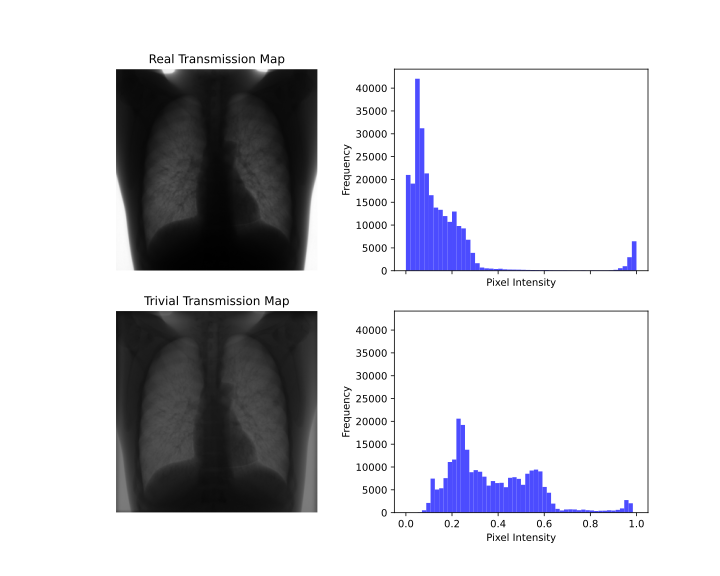
\includegraphics[width=0.8\textwidth]{figures/trivial_histogram.png}
    \caption{Example of trivial inversion transformation and the corresponding histogram. The inversion is computed
    from the paired processed image of the shown image.}
    \label{fig:trivial_inversion}
\end{figure}

\section{Experiment Methodology}

Let's recall that there are two core cases of the optimization problem proposed. One consists of solving an optimization problem
on a per-image basis, assuming there is no set of parameters that can map a plausible transmission map to the processed image.
Note that, in terms of implementation, it is possible to solve multiple optimization problems at once to speed up computing.
For this case, the hyperparameter search is done by choosing a new set of parameters and performing the minimization algorithm
for a small set of images at once, and repeating it for other sets of images. Evaluation metrics are then aggregated across all the
seen images and iterations. The batches of images and iterations are kept small to speed up the computation, specifically,
batches of 4 images for 4 different batches. For validation, a larger set of images is used to evaluate the scaling suitability
of the chosen parameters.

The second approach is to find a single set of parameters that can produce a valid solution for all images.
The approach taken in this case is analogous to the first one. However, there is a significant difference that image
updates are not independent, since the updates of $\theta$ will aim to reduce the loss across the selected subset.

The expected outcome of the implementation is to find a set of hyperparameters and a concrete model (e.g., choosing the
proper smoothing regularization) that can be used to solve the inverse problem for any given image without any further tuning,
and ideally, in an efficient manner. For the selection of the optimal hyperparameters, there are certain considerations that may
conflict with each other. The ideal model should

\begin{itemize}
    \item recover the processed images accurately,
    \item recover transmission maps with values within the restricted physical bounds, and
    \item be computationally efficient.
\end{itemize}

Regarding measuring the fidelity of the processed images, it was mentioned previously that \arcshort{MSE} does not necessarily favor
solutions that are perceptually close to the original images. The $\matchal{L}^{\text{Mix}}$ loss \cite{zhaoLossFunctionsImage2017}
can be a suitable choice for evaluating the results and discerning the best choice of hyperparameters.
A detailed description of the function can be found in \autoref{app:mixLoss}. The next chapter will also present further
insights on this choice.

As for ensuring the physical bounds, it is addressed by computing the total square error of the transmission maps
and aiming to minimize the error simultaneously. Finally, a set of hyperparameters that can reduce the overall number of
iterations to converge is preferred.


\chapter{Results and Analysis}
\label{ch:resultsAndAnalysis}

This chapter covers the results of the multiple hyperparameter searches done, as well as
quantitative and qualitative insights on the performance of the model.

\section{Data Fidelity}

In the last section, the loss $\mathcal{L}^{\text{Mix}}$ was mentioned as the core evaluation metric for the model performance,
in terms of the quality of the recovered transmission maps and the estimated processed images. Evidence of the suitability
of this metric is shown in \autoref{fig:transmission_maps}.

\begin{figure}[ht]
    \centering
    \includegraphics[width=1.0\textwidth]{figures/L_mix.png}
    \caption{The data points in the scatter plots represent different optimization runs and the average of the metric values
    (MSE, SSIM, $\mathcal{L}$) over the images used on each run. It can be observed a correlation of $\mathcal{L}^{\text{Mix}}$,
    As SSIM approaches one, and MSE approaches zero, the value gets closer to zero. However, $\mathcal{L}^{\text{Mix}}$
    converges at a much slower rate than the other metrics.}
    \label{fig:transmission_maps}
\end{figure}

\section{Per-image optimization}

An initial set of hyperparameter searches was set out to perform the choice of a smoothing regularization, as well as a preliminary
choice of regularization parameters. Three separate searches were done for each type of smoothing regularization:
no regularization, Tikhonov regularization, and Total Variation. The consideration of this type of regularization came up during
initial experiments, where reconstructed images were found to be noisy and presented artifacts, such as the ones in
\autoref{fig:artifacts}. The list of the best evaluation scores across these searches is shown in \autoref{tab:hyperparameterSearch}.

\begin{figure}[ht]
    \centering
    \includegraphics[width=0.7\textwidth]{figures/noisy.png}
    \caption{Reconstructed processed image with noise artifacts.}
    \label{fig:artifacts}
\end{figure}

The latest searches were set to optimize parameters relative to the $\mathcal{L}^{\text{Mix}}$ loss, and out of the three methods, the one
that achieved the best score was using no regularization. Even though the regularization terms converge to parameters
that yield low reconstruction errors, the choice of parameters for both regularization terms introduced
shadow artifacts around the segmentation regions as seen in \autoref{fig:shadowArtifacts}. The reason for not needing
a smoothing regularization could come from the initialization of images with their trivial transformation, which
can be seen as a close approximation of the transmission map. This initialization was different in initial experiments,
defaulting to the original images or random noise. Ultimately, this initialization was found to converge faster.

\begin{figure}[ht]
    \centering
    \includegraphics[width=0.7\textwidth]{figures/shadowed.png}
    \caption{Reconstructed processed image with shadow artifacts.}
    \label{fig:shadowArtifacts}
\end{figure}

Using the parameters that led to a lower loss on a larger set of images for validation, the quality in the reconstructed
processed images remained consistent, as well as the compliance with the anatomical bounds. A full overview of the results can
be seen in \autoref{app:initialParamsResults}. However, few cases on the transmission maps showed hard edges in the outline of the body depicted
in \autoref{fig:outlineArtifacts}.


\begin{figure}[!tbp]
  \centering
  \begin{minipage}[b]{0.4\textwidth}
    \includegraphics[width=\textwidth]{figures/outline1.png}
  \end{minipage}
  \hfill
  \begin{minipage}[b]{0.4\textwidth}
    \includegraphics[width=\textwidth]{figures/outline2.png}
  \end{minipage}
  \caption{Example of transmission maps presenting glowing edges.}
  \label{fig:outlineArtifacts}
\end{figure}


\section{Further parameter search}

The model considers other parameters besides the regularization terms and optimization terms, such as learning rates.
These refer to the box constraints set on the processing function. These are initially set based on empirical evidence,
such as suggestions of kernel sizes based on the real size of edges in radiographies. These constraints are set to inject
prior information about the minimal transformations expected in the image processing pipeline. Choosing these values without
care can lead to seemingly valid reconstructions, but can characterize the reconstructed transmission maps to be
unrealistic. Consider the case depicted in \autoref{fig:wrongCharacterization} of using an optimal choice of hyperparameters,
but constraining the lower bound of an enhancement factor too high in the high-frequencies. The processed image can
be perceived as a close reconstruction of the original image, but the transmission map is overly smooth, which is unlikely
to be a realistic representation.

\begin{figure}[ht]
  \centering
  \begin{minipage}[b]{0.4\textwidth}
    \includegraphics[width=\textwidth]{figures/wrong_character_tm.png}
  \end{minipage}
  \begin{minipage}[b]{0.4\textwidth}
    \includegraphics[width=\textwidth]{figures/wrong_character_proc.png}
  \end{minipage}
  \hfill
  \caption{Example of a recovered transmission map and its estimated processed version using a minimum enhancement factor
  of 0.59 in the low-frequencies, and setting 3.95 as the std. for such frequency bands.}
  \label{fig:wrongCharacterization}
\end{figure}

These, nevertheless, are based on assumptions and no solid data. They can also be hard to set since they can
depend on the image size. A straightforward way to adjust these constraints is to pick an optimal set of
hyperparameters and perform once again a parameter search, specifically to fix these bounds. The objective is to find parameters
that can minimize the error with the known ground truth. This method keeps the data fidelity errors low, as
the original hyperparameters. Specific metrics and examples are presented in \autoref{app:refinedParamsResults}.

\begin{table}[H]
\centering
\begin{tabular}{ | c | c| }
\hline \\
Parameter & Value \\
\hline \\
Low-frequency std. & 28.033104695552467 \\
\hline \\
Minimum Low-frequency enhancement factor in low frequencies & 0.23209908549082872 \\
\hline \\
High-frequency std. & 2.5834306818846415 \\
\hline \\
Minimum High-frequency enhancement factor in high frequencies & 0.4323876961409312 \\
\hline
\end{tabular}
\caption{Found parameters for frequency band constraints.}
\end{table}

\section{Common parameters optimization}

An alternative approach to implementing the optimization solver is to update a single set of parameters across all images.
This can be done by using a single loss function that combines the losses of all images and updating the parameters
using a single optimizer. This approach showed poor performance, failing to converge to a set of hyperparameters
that reduce the Mixed loss sufficiently, and also showed a trend to produce images with flat regions as seen in \autoref{fig:flatRegions}.

\begin{figure}[H]
\centering
\includegraphics[width=0.7\textwidth]{figures/flat_regions.png}
\caption{Sample recovered transmission map image with flat regions.}
\label{fig:flatRegions}
\end{figure}

An alternative approach, suggested by the proximity of parameters recovered by previous experiments (see \autoref{fig:parameterDistribution}),
hinted that a single choice of processing parameters can effectively map back to a realistic transmission map.
That idea can be proved by picking a set of parameters returned from an optimization run, and setting it as the initial
weights and freezing their updates. An experiment proved this possible. Nonetheless, there is no noticeable
performance improvement, inverting 96 images in 44 minutes (1 image every ~27 seconds). This suggests the parameters
converge at a much higher rate than the transmission map images, although a few images stuck in the iteration process
can also be a reason for the high runtime.

\begin{figure}[h]
\centering
\includegraphics[width=1.0\textwidth]{figures/weights_boxplot.png}
\caption{Distribution of the processing function parameters from 200 reconstructed transmission maps.}
\label{fig:parameterDistribution}
\end{figure}

\cleardoublepage
\chapter{Conclusions and Future Work}
\label{ch:conclusionsAndFutureWork}

\section{Summary of Contributions}

This thesis addressed a critical challenge in medical imaging: the significant appearance variability in chest X-ray datasets caused by diverse acquisition systems and proprietary image processing pipelines. This diversity limits the generalization of diagnostic learning models, particularly affecting alternative X-ray detectors that are underrepresented in major datasets. The implications extend beyond technical limitations, as these alternative systems often represent the only viable diagnostic option in resource-limited settings, making this a matter of healthcare equity.

We successfully recovered transmission maps from processed clinical X-ray images without access to the manufacturer's proprietary algorithms or paired training data. Our constrained optimization approach exploited the fact that all clinical processing pipelines share common goals to infer plausible inverse transformations. The recovered transmission maps not only produced accurate reconstructions when re-processed but also exhibited the physical characteristics expected from real X-ray attenuation data, including appropriate tissue-specific absorption values and the absence of enhancement artifacts present in processed images.


\section{Technical Achievements and Limitations}

The physics-informed approach developed in this work successfully models the forward processing pipeline as a composition of fundamental operations, including negative logarithm transformation, windowing, and multi-scale unsharp masking. This modeling choice, validated through close correspondence between reconstructed and original clinical images, confirms our understanding of the essential transformations applied in commercial systems despite their proprietary nature.

However, the current implementation faces a significant computational challenge that limits its immediate practical application. Each image requires an independent optimization process involving hundreds of iterations to achieve convergence. This computational burden makes the processing of large-scale datasets impractical with current resources. Furthermore, the method does not yield a generalizable transformation operator that can be directly applied to new images. Instead, each optimization may converge to different processing parameters, preventing the extraction of a unified inverse model.

The validation of our approach remains constrained by the availability of only a single ground truth transmission map-processed image pair. While the method demonstrates consistent performance across images from standard datasets, comprehensive validation of transmission map accuracy would benefit from additional ground truth data. The optimization landscape also presents challenges, containing multiple local minima that make results sensitive to initialization strategies and hyperparameter choices, particularly in balancing the weights between smoothness constraints and anatomical priors.

Despite these limitations, this work establishes important foundations for advancing medical imaging accessibility. The demonstrated feasibility of transmission map recovery provides a potential pathway for leveraging existing annotated datasets with alternative imaging systems. This capability could accelerate the deployment of AI-assisted diagnosis in underserved regions where conventional high-end imaging systems are unavailable or impractical.

The physics-informed methodology presented here also contributes to the broader discourse on incorporating domain knowledge into machine learning systems. In an era dominated by purely data-driven approaches, our work demonstrates that the careful integration of physical constraints can effectively guide solutions in under-constrained problems, offering a complementary paradigm that is particularly valuable when training data is scarce.

\section{Concluding Remarks}



While computational efficiency remains a challenge, the framework established here provides both a proof of concept and a benchmark for future developments. As healthcare systems worldwide continue to grapple with issues of accessibility and equity, approaches that can bridge the gap between high-end imaging systems and resource-appropriate alternatives become increasingly vital. By enabling the potential translation of existing medical knowledge to new imaging contexts, this research contributes to the broader goal of universal access to healthcare diagnostics.




\cleardoublepage
% Print the bibliography (and make it appear in the table of contents)
\renewcommand{\bibname}{References}


\ifbiblatex
    %\typeout{Biblatex current language is \currentlang}
    \printbibliography[heading=bibintoc]
\else
    \phantomsection  % make it include a hyperref - see https://tex.stackexchange.com/a/98995
    \addcontentsline{toc}{chapter}{References}
    \bibliography{references}
\fi



% \warningExpl{If you do not have an appendix, do not include the \textbackslash cleardoublepage command below; otherwise, the last page number in the metadata will be one too large.}
% \cleardoublepage
\appendix
\renewcommand{\chaptermark}[1]{\markboth{Appendix \thechapter\relax:\thinspace\relax#1}{}}
\chapter{Supporting Material}
% \label{sec:supportingMaterial}

\begin{figure}
    \centering
    \includegraphics[width=1.0\textwidth]{figures/window_params.png}
    \caption{Windowing function with different parameter settings.}
    \label{fig:windowingParams}
\end{figure}

\begin{algorithm}[htbp]
\scriptsize
\SetAlgoLined
% \DontPrintSemicolon
\allowdisplaybreaks
\setlength{\algomargin}{5pt}
\sloppy
\KwIn{$pred$ - Batch of prediction masks with shape (batch, labels, height, width)}
\KwIn{$threshold$ - Optional threshold value}
\KwOut{$ordered\_groups$ - List of mask group identifiers}
\KwOut{$exclusive\_masks$ - Array of exclusive masks with shape (batch, reduced\_labels, height, width)}

\BlankLine
\SetKwFunction{FBatchGetExclusiveMasks}{BatchGetExclusiveMasks}
\SetKwProg{Fn}{Function}{:}{}
\Fn{\FBatchGetExclusiveMasks{$pred$, $threshold$}}{
    $complete\_masks \leftarrow [$ $]$\;

    \ForEach{$group \in \text{MASK\_GROUPS}$}{
        $group\_mask \leftarrow \text{GetGroupMask}(pred, group, threshold)$\;

        Concatenate on labels axis $group\_mask$ to $complete\_masks$\;
    }

    \BlankLine
    $exclusive\_masks \leftarrow \text{Copy}(complete\_masks)$\;

    $groups\_count \leftarrow \text{len}(\text{MASK\_GROUPS})$\;

    \tcc{Masks are substracted in specific order, denser groups last}

    \For{$i \leftarrow 0$ \KwTo $groups\_count - 1$}{
        \For{$j \leftarrow 0$ \KwTo $groups\_count -1$}{
            \If{$j < i$}{
                \tcc{Subtract already exclusive masks}
                $exclusive\_masks[:, i] \leftarrow \text{SubtractMask}($\\
                \hspace*{2.5cm}$exclusive\_masks[:, i], exclusive\_masks[:, j])$\;
            }
            \eIf{$j > i$}{
                \tcc{Subtract entire masks}
                $exclusive\_masks[:, i] \leftarrow \text{SubtractMask}($\\
                \hspace*{2.5cm}$exclusive\_masks[:, i], complete\_masks[:, j])$\;
            }
        }
    }
    \KwRet{$exclusive\_masks$}\;
}

\BlankLine
\SetKwFunction{FGetGroupMask}{GetGroupMask}
\Fn{\FGetGroupMask{$pred$, $group$, $threshold$}}{
    \tcc{Select only the labels in the group}

    $group\_masks \leftarrow \text{FilterPredMasks}(pred, group)$\;

    $normalized\_masks \leftarrow \text{Sigmoid}(group\_masks)$\;

    \tcc{Indicator function: 1 where condition is true, 0 otherwise}

    $thresholded\_masks \leftarrow \mathbbm{1}\{normalized\_masks > threshold\}$\;

    $joined\_masks \leftarrow \text{sum}(thresholded\_masks, axis=1)$\;

    \KwRet{$\text{clip}(thresholded\_masks, 0.0, 1.0)$}\;
}

\caption{Algorithms for creating exclusive segmentation masks}
\label{alg:mergeSegmentationMasks}
\end{algorithm}
\vspace{-3mm}


\chapter{Initial hyperparameter search}
\label{sec:initialHyperparameterSearch}

\begin{sidewaystable}
\centering
\begin{tabularx}{\linewidth}{lrrrrrrrl}
 & Runtime & $\mathcal{L}^{\text{Mix}}$ max & $\mathcal{L}^{\text{Mix}}$ mean & $\mathcal{L}^{\text{Mix}}$ min & Penalties max & Penalties mean & Penalties min & Smooth reg. \\
 29 & 563.109801 & \bfseries 0.016853 & \bfseries 0.014564 & \bfseries 0.012100 & \bfseries 0.003202 & \bfseries 0.001207 & 0.000044 & none \\
 30 & 1071.619600 & 0.018997 & 0.016656 & 0.013023 & 0.003599 & 0.001449 & 0.000052 & none \\
 34 & 1017.985566 & 0.027841 & 0.024338 & 0.018678 & 0.004580 & 0.002035 & 0.000077 & none \\
 12 & 699.119695 & 0.030976 & 0.027394 & 0.023818 & 0.017649 & 0.003872 & 0.000143 & tikhonov \\
 18 & 476.124311 & 0.036701 & 0.033039 & 0.029165 & 0.029165 & 0.012455 & 0.000625 & tikhonov \\
 21 & 475.003554 & 0.054005 & 0.049602 & 0.046968 & 0.242348 & 0.156652 & 0.017277 & tikhonov \\
 0 & 713.010703 & 0.058910 & 0.053848 & 0.049643 & 0.020831 & 0.010680 & 0.000624 & tv \\
 3 & 970.882263 & 0.060052 & 0.054773 & 0.047618 & 0.523728 & 0.309372 & 0.044149 & tv \\
 8 & 539.165788 & 0.059271 & 0.055080 & 0.052517 & 1.536641 & 0.989059 & 0.135147 & tv \\
 5 & 245.019457 & 0.059813 & 0.055580 & 0.051776 & 0.054485 & 0.026585 & 0.001869 & tv \\
 17 & 468.220039 & 0.065625 & 0.060227 & 0.054002 & 0.048943 & 0.027634 & 0.003310 & tikhonov \\
 10 & 368.075797 & 0.068312 & 0.064878 & 0.059608 & 0.951185 & 0.535663 & 0.066518 & tv \\
 7 & 376.274129 & 0.075618 & 0.070741 & 0.066959 & 0.058924 & 0.032396 & 0.003098 & tv \\
 16 & 661.980748 & 0.076345 & 0.071043 & 0.064878 & 0.030261 & 0.017630 & 0.002333 & tikhonov \\
 20 & 605.175529 & 0.080235 & 0.074267 & 0.068925 & 0.067765 & 0.039111 & 0.006383 & tikhonov \\
 32 & 687.701262 & 0.085997 & 0.076598 & 0.069191 & 0.012257 & 0.006835 & 0.000804 & none \\
 1 & 595.768241 & 0.226541 & 0.098334 & 0.053218 & 0.583420 & 0.351899 & 0.000231 & tv \\
 27 & 730.086226 & 0.344054 & 0.100650 & 0.015107 & 0.005781 & 0.002064 & \bfseries 0.000000 & none \\
 2 & 514.845521 & 0.255809 & 0.111593 & 0.054730 & 0.078831 & 0.049376 & \bfseries 0.000000 & tv \\
 4 & 717.700773 & 0.197577 & 0.115705 & 0.033487 & 119.200302 & 28.410555 & 0.982594 & tv \\
 9 & \bfseries 244.023881 & 0.310923 & 0.117600 & 0.045247 & 0.254540 & 0.129439 & 0.000000 & tv \\
 15 & 784.657229 & 0.127563 & 0.121181 & 0.113680 & 0.155192 & 0.085257 & 0.013254 & tikhonov \\
 23 & 461.161033 & 0.370886 & 0.122585 & 0.033377 & 0.084576 & 0.022226 & 0.000004 & tikhonov \\
 26 & 692.708670 & 0.129267 & 0.122605 & 0.114367 & 0.051751 & 0.029769 & 0.005660 & none \\
 33 & 756.872708 & 0.141169 & 0.130073 & 0.116452 & 0.040259 & 0.022843 & 0.004338 & none \\
 14 & 287.046453 & 0.147056 & 0.135629 & 0.124201 & 0.451391 & 0.267444 & 0.129689 & tikhonov
 \end{tabularx}
\caption{Initial hyperparameter search results, ordered by the average $\mathcal{L}$.
The table also includes penalty values, which correspond to the total sum of the
segmentation penalties (averaged over all images), smoothing regularization, and the
total runtime used (in seconds).}
\label{tab:hyperparameterSearch}
\end{sidewaystable}

\chapter{Mix Loss Function}
\label{app:mixLoss}

The $\mathcal{L}^{\text{Mix}}$ loss function used for evaluation in this work combines the perceptual advantages of \acrfull{MS-SSIM} with the stability of the $\ell_1$ loss. As proposed by Zhao et al. \cite{zhaoLossFunctionsImage2017}, this hybrid loss function is defined as:

\begin{equation}
\mathcal{L}^{\text{Mix}} = \alpha \cdot \mathcal{L}^{\text{MS-SSIM}} + (1 - \alpha) \cdot \mathcal{L}_1
\label{eq:mixLoss}
\end{equation}

where $\alpha \in [0, 1]$ is a weighting parameter that balances the contribution of each component. The optimal value $\alpha = 0.84$ was determined empirically across various image restoration tasks.

The MS-SSIM loss component is derived from the Multi-Scale Structural Similarity index by converting it to a loss form:

\begin{equation}
\mathcal{L}^{\text{MS-SSIM}} = 1 - \text{MS-SSIM}(x, y)
\end{equation}

The MS-SSIM index itself evaluates image similarity at multiple scales through:

\begin{equation}
\text{MS-SSIM}(x, y) = [l_M(x, y)]^{\alpha_M} \cdot \prod_{j=1}^{M} [c_j(x, y)]^{\beta_j} [s_j(x, y)]^{\gamma_j}
\end{equation}

where $M$ denotes the number of scales, and the components at each scale $j$ are defined as:

\begin{align}
l_j(x, y) &= \frac{2\mu_x\mu_y + C_1}{\mu_x^2 + \mu_y^2 + C_1} \quad \text{(luminance comparison)}\\
c_j(x, y) &= \frac{2\sigma_x\sigma_y + C_2}{\sigma_x^2 + \sigma_y^2 + C_2} \quad \text{(contrast comparison)}\\
s_j(x, y) &= \frac{\sigma_{xy} + C_3}{\sigma_x\sigma_y + C_3} \quad \text{(structure comparison)}
\end{align}

Here, $\mu_x$ and $\mu_y$ are the mean intensities, $\sigma_x$ and $\sigma_y$ are the standard deviations, and $\sigma_{xy}$ is the covariance between images $x$ and $y$ at scale $j$. The constants $C_1$, $C_2$, and $C_3$ provide numerical stability. The exponents $\{\alpha_M, \beta_j, \gamma_j\}$ weight the relative importance of each component, with typical values being $\alpha_M = \beta_M = \gamma_M = 1$ and normalized  $\sum_{j=1}^M \gamma_j = 1$ \cite[p.~1399]{wangMultiscaleStructuralSimilarity2003}.

The $\ell_1$ loss component provides the mean absolute error:

\begin{equation}
\mathcal{L}_1 = \frac{1}{N} \sum_{i=1}^{N} |x_i - y_i|
\end{equation}

where $N$ is the total number of pixels in the image. This component ensures pixel-level fidelity and helps preserve color and brightness information that might be underweighted by the MS-SSIM component alone.

The combination of these two losses leverages MS-SSIM's ability to capture perceptual similarity across multiple scales—aligning with how the human visual system processes images—while the $\ell_1$ term provides optimization stability and prevents color shifts. This makes $\mathcal{L}^{\text{Mix}}$ particularly effective for image reconstruction tasks where both perceptual quality and pixel accuracy are critical.

\chapter{Initial Parameter Search Results}
\label{app:initialParamsResults}

The recovered transmission map scores $\mathcal{L}^{\text{Mix}} = 0.276278555393219$.
The trivial transmission map scores $\mathcal{L}^{\text{Mix}} = 0.4022318422794342$

\begin{figure}[H]
\centering
\includegraphics[width=1.0\textwidth]{figures/initial/pred_ms_ssim_percentiles.png}
\caption{Sample images at percentiles of $\mathcal{L}^{\text{Mix}}$ }
\end{figure}

\begin{figure}[H]
\centering
\includegraphics[width=1.0\textwidth]{figures/initial/histogram_heatmap.png}
\caption{Histograms of recovered transmission maps, sampled 200 images.}
\end{figure}

\begin{figure}[H]
\centering
\includegraphics[width=1.0\textwidth]{figures/initial/cmp_histogram.png}
\caption{Comparison of histograms between trivial, real, and predicted transmission maps.}
\end{figure}


\chapter{Refined Parameter Search Results}
\label{app:refinedParamsResults}

The recovered transmission map scores $\mathcal{L}^{\text{Mix}} = 0.2652566134929657$..
The trivial transmission map scores $\mathcal{L}^{\text{Mix}} = 0.4022318422794342$

\begin{figure}[H]
\centering
\includegraphics[width=1.0\textwidth]{figures/further/pred_ms_ssim_percentiles.png}
\caption{Sample images at percentiles of $\mathcal{L}^{\text{Mix}}$ }
\end{figure}

\begin{figure}[H]
\centering
\includegraphics[width=1.0\textwidth]{figures/further/histogram_heatmap.png}
\caption{Histograms of recovered transmission maps, sampled 200 images.}
\end{figure}

\begin{figure}[H]
\centering
\includegraphics[width=1.0\textwidth]{figures/further/cmp_histogram.png}
\caption{Comparison of histograms between trivial, real, and predicted transmission maps.}
\end{figure}

% \generalExpl{Here is a place to add supporting material that can help others build upon your work. You can include files as attachments to the PDF file or indirectly via URLs. Alternatively, consider adding supporting material uploaded as separate files in DiVA.}

% Attach the BibTeX for your references to make it easy for a reader to find and use them
% The BibTeX references used in this thesis are attached. \attachfile[description={references.bib}]{references.bib}

% % Attach source code file(s) or add a URL to the github or other repository
% Some source code relevant to this project can be found at \url{https://github.com/gqmaguirejr/E-learning} and \url{https://github.com/gqmaguirejr/Canvas-tools}.

% Your reader can access the attached (embedded) files using a PDF tool such as Adobe Acrobat Reader using the paperclip icon in the left menu, as shown in \Cref{fig:PDFreaderPaperclipExample} or by right-clicking on the push-pin icon in the PDF file and then using the menu to save the embedded file as shown in \Cref{fig:PDFreaderPushpinExample}.

% An argument for including supporting material in the PDF file is that it will be available to anyone who has a copy of the PDF file. As a result, they do not have to look elsewhere for this material. This comes at the cost of a larger PDF file. However, the embedded files are encoded into a compressed stream within the PDF file; thus, reducing the number of additional bytes. For example, the references.bib file that was used in this example is \SI{10617}{\byte} in size but only occupies \SI{4261}{\byte} in the PDF file.

% \warningExpl{DiVA is limited to $\approx$\SI{1}{\giga\byte} for each supporting file. If you have very large amounts of supporting material, you will probably want to use one of the data repositories. For additional help with this, contact KTH Library via
% \href{mailto:researchdata@kth.se}{researchdata@kth.se}.\\As of Spring 2024, there are plans to migrate this supporting data from DiVA to a research data repository.
% }

% \begin{figure}[!ht]
%   \begin{center}
%     \includegraphics[width=0.50\textwidth]{README_notes/pdf-viewer-attached-files.png}
%   \end{center}
%   \caption{Adobe Acrobat Reader using the paperclip icon for the attached references.bib file}
%   \label{fig:PDFreaderPaperclipExample}
% \end{figure}
% \FloatBarrier

% \begin{figure}[!ht]
%   \begin{center}
%     \includegraphics[width=0.99\textwidth]{README_notes/Bib-save-embedded-example.png}
%   \end{center}
%   \caption{Adobe Acrobat Reader after right-clicking on the push-pin icon for the attached references.bib file}
%   \label{fig:PDFreaderPushpinExample}
% \end{figure}
% \FloatBarrier
% \cleardoublepage

% \chapter{Something Extra}
% \sweExpl{svensk: Extra Material som Bilaga}


% \textcolor{black}{black} {\color{black} \rule{\linewidth}{1mm} }

% % Include an example of using nomenclature
% \ifnomenclature
%     \cleardoublepage
%     \chapter{Main equations}
%     \label{ch:NomenclatureExamples}
%     This appendix gives some examples of equations that are used throughout this thesis.
%     \section{A simple example}
%     The following example is adapted from Figure 1 of the documentation for the package nomencl (\url{https://ctan.org/pkg/nomencl}).
%     \begin{equation}\label{eq:mainEq}
%     a=\frac{N}{A}
%     \end{equation}
%     \nomenclature{$a$}{The number of angels per unit area\nomrefeq}%       %% include the equation number in the list
%     \nomenclature{$N$}{The number of angels per needle point\nomrefpage}%  %% include the page number in the list
%     \nomenclature{$A$}{The area of the needle point}%
%     The equation $\sigma = m a$%
%     \nomenclature{$\sigma$}{The total mass of angels per unit area\nomrefeqpage}%
%     \nomenclature{$m$}{The mass of one angel}
% follows easily from \Cref{eq:mainEq}.

%     \section{An even simpler example}
%     The formula for the diameter of a circle is shown in \Cref{eq:secondEq} area of a circle in \cref{eq:thirdEq}.
%     \begin{equation}\label{eq:secondEq}
%     D_{circle}=2\pi r
%     \end{equation}
%     \nomenclature{$D_{circle}$}{The diameter of a circle\nomrefeqpage}%
%     \nomenclature{$r$}{The radius of a circle\nomrefeqpage}%

%     \begin{equation}\label{eq:thirdEq}
%     A_{circle}=\pi r^2
%     \end{equation}
%     \nomenclature{$A_{circle}$}{The area of a circle\nomrefeqpage}%

%     Some more text that refers to \eqref{eq:thirdEq}.
% \fi  %% end of nomenclature example

% \cleardoublepage
% % Information for authors
% %\include{README_author}
% \subfile{README_author}

% \cleardoublepage
% % information about the template for everyone
% \input{README_notes/README_notes}

\begin{comment}
% information for examiners
\ifxeorlua
\cleardoublepage
\input{README_notes/README_examiner_notes}
\fi
\end{comment}

\begin{comment}
% Information for administrators
\ifxeorlua
\cleardoublepage
\input{README_notes/README_for_administrators.tex}
\fi
\end{comment}

\begin{comment}
% Information for Course Coordinators
\ifxeorlua
\cleardoublepage
\input{README_notes/README_for_course_coordinators}
\fi
\end{comment}

%% The following label is necessary for computing the last page number of the body of the report to include in the "For DIVA" information
\label{pg:lastPageofMainmatter}

\cleardoublepage
\clearpage\thispagestyle{empty}\mbox{} % empty page with backcover on the other side
\kthbackcover
\fancyhead{}  % Do not use header on this extra page or pages
\section*{€€€€ For DIVA €€€€}
\lstset{numbers=none} %% remove any list line numbering
\divainfo{pg:lastPageofPreface}{pg:lastPageofMainmatter}

% If there is an acronyms.tex file,
% add it to the end of the For DIVA information
% so that it can be used with the abstracts
% Note that the option "nolol" stops it from being listed in the List of Listings

% The following bit of ugliness is because of the problems PDFLaTeX has handling a non-breaking hyphen
% unless it is converted to UTF-8 encoding.
% If you do not use such characters in your acronyms, this could be simplified.
\ifxeorlua
\IfFileExists{lib/acronyms.tex}{
\section*{acronyms.tex}
\lstinputlisting[language={[LaTeX]TeX}, nolol, basicstyle=\ttfamily\color{black},
commentstyle=\color{black}, backgroundcolor=\color{white}]{lib/acronyms.tex}
}
{}
\else
\IfFileExists{lib/acronyms-for-pdflatex.tex}{
\section*{acronyms.tex}
\lstinputlisting[language={[LaTeX]TeX}, nolol, basicstyle=\ttfamily\color{black},
commentstyle=\color{black}, backgroundcolor=\color{white}]{lib/acronyms-for-pdflatex.tex}
}
{}
\fi


\end{document}
